\documentclass[]{book}
%%%%%%%%%%%%%%%%%%%%%%%%%%%%%%%%%%%%%%%%%
% The Legrand Orange Book
% Structural Definitions File
% Version 2.1 (26/09/2018)
%
% Original author:
% Mathias Legrand (legrand.mathias@gmail.com) with modifications by:
% Vel (vel@latextemplates.com)
% 
% This file was downloaded from:
% http://www.LaTeXTemplates.com
%
% License:
% CC BY-NC-SA 3.0 (http://creativecommons.org/licenses/by-nc-sa/3.0/)
%
%%%%%%%%%%%%%%%%%%%%%%%%%%%%%%%%%%%%%%%%%

%----------------------------------------------------------------------------------------
%	VARIOUS REQUIRED PACKAGES AND CONFIGURATIONS
%----------------------------------------------------------------------------------------

\usepackage{graphicx} % Required for including pictures
\graphicspath{{./poly/Pictures/}} % Specifies the directory where pictures are stored

\usepackage{lipsum} % Inserts dummy text

\usepackage{tikz} % Required for drawing custom shapes


\usepackage{enumitem} % Customize lists
\setlist{nolistsep} % Reduce spacing between bullet points and numbered lists

\usepackage{booktabs} % Required for nicer horizontal rules in tables

\usepackage{xcolor} % Required for specifying colors by name
\definecolor{ocre}{RGB}{243,102,25} % Define the orange color used for highlighting throughout the book

%----------------------------------------------------------------------------------------
%	MARGINS
%----------------------------------------------------------------------------------------

\usepackage{geometry} % Required for adjusting page dimensions and margins

\geometry{
	paper=a4paper, % Paper size, change to letterpaper for US letter size
	top=3cm, % Top margin
	bottom=3cm, % Bottom margin
	left=3cm, % Left margin
	right=3cm, % Right margin
	headheight=14pt, % Header height
	footskip=1.4cm, % Space from the bottom margin to the baseline of the footer
	headsep=10pt, % Space from the top margin to the baseline of the header
	%showframe, % Uncomment to show how the type block is set on the page
}

%----------------------------------------------------------------------------------------
%	FONTS
%----------------------------------------------------------------------------------------

\usepackage{avant} % Use the Avantgarde font for headings
%\usepackage{times} % Use the Times font for headings
\usepackage{mathptmx} % Use the Adobe Times Roman as the default text font together with math symbols from the Sym­bol, Chancery and Com­puter Modern fonts

\usepackage{microtype} % Slightly tweak font spacing for aesthetics

%----------------------------------------------------------------------------------------
%	BIBLIOGRAPHY AND INDEX
%----------------------------------------------------------------------------------------
\usepackage{csquotes}
\usepackage[style=numeric,citestyle=numeric,sorting=nyt,sortcites=true,autopunct=true,autolang=hyphen,hyperref=true,abbreviate=false,backref=true,backend=biber]{biblatex}
\addbibresource{bibliography.bib} % BibTeX bibliography file
\defbibheading{bibempty}{}

\usepackage{calc} % For simpler calculation - used for spacing the index letter headings correctly
\usepackage{makeidx} % Required to make an index
\makeindex % Tells LaTeX to create the files required for indexing

%----------------------------------------------------------------------------------------
%	MAIN TABLE OF CONTENTS
%----------------------------------------------------------------------------------------

\usepackage{titletoc} % Required for manipulating the table of contents

\contentsmargin{0cm} % Removes the default margin

% Part text styling (this is mostly taken care of in the PART HEADINGS section of this file)
\titlecontents{part}
	[0cm] % Left indentation
	{\addvspace{20pt}\bfseries} % Spacing and font options for parts
	{}
	{}
	{}

% Chapter text styling
\titlecontents{chapter}
	[1.25cm] % Left indentation
	{\addvspace{12pt}\large\sffamily\bfseries} % Spacing and font options for chapters
	{\color{ocre!60}\contentslabel[\Large\thecontentslabel]{1.25cm}\color{ocre}} % Formatting of numbered sections of this type
	{\color{ocre}} % Formatting of numberless sections of this type
	{\color{ocre!60}\normalsize\;\titlerule*[.5pc]{.}\;\thecontentspage} % Formatting of the filler to the right of the heading and the page number

% Section text styling
\titlecontents{section}
	[1.25cm] % Left indentation
	{\addvspace{3pt}\sffamily\bfseries} % Spacing and font options for sections
	{\contentslabel[\thecontentslabel]{1.25cm}} % Formatting of numbered sections of this type
	{} % Formatting of numberless sections of this type
	{\hfill\color{black}\thecontentspage} % Formatting of the filler to the right of the heading and the page number

% Subsection text styling
\titlecontents{subsection}
	[1.25cm] % Left indentation
	{\addvspace{1pt}\sffamily\small} % Spacing and font options for subsections
	{\contentslabel[\thecontentslabel]{1.25cm}} % Formatting of numbered sections of this type
	{} % Formatting of numberless sections of this type
	{\ \titlerule*[.5pc]{.}\;\thecontentspage} % Formatting of the filler to the right of the heading and the page number

% Figure text styling
\titlecontents{figure}
	[1.25cm] % Left indentation
	{\addvspace{1pt}\sffamily\small} % Spacing and font options for figures
	{\thecontentslabel\hspace*{1em}} % Formatting of numbered sections of this type
	{} % Formatting of numberless sections of this type
	{\ \titlerule*[.5pc]{.}\;\thecontentspage} % Formatting of the filler to the right of the heading and the page number

% Table text styling
\titlecontents{table}
	[1.25cm] % Left indentation
	{\addvspace{1pt}\sffamily\small} % Spacing and font options for tables
	{\thecontentslabel\hspace*{1em}} % Formatting of numbered sections of this type
	{} % Formatting of numberless sections of this type
	{\ \titlerule*[.5pc]{.}\;\thecontentspage} % Formatting of the filler to the right of the heading and the page number

%----------------------------------------------------------------------------------------
%	MINI TABLE OF CONTENTS IN PART HEADS
%----------------------------------------------------------------------------------------

% Chapter text styling
\titlecontents{lchapter}
	[0em] % Left indentation
	{\addvspace{15pt}\large\sffamily\bfseries} % Spacing and font options for chapters
	{\color{ocre}\contentslabel[\Large\thecontentslabel]{1.25cm}\color{ocre}} % Chapter number
	{}  
	{\color{ocre}\normalsize\sffamily\bfseries\;\titlerule*[.5pc]{.}\;\thecontentspage} % Page number

% Section text styling
\titlecontents{lsection}
	[0em] % Left indentation
	{\sffamily\small} % Spacing and font options for sections
	{\contentslabel[\thecontentslabel]{1.25cm}} % Section number
	{}
	{}

% Subsection text styling (note these aren't shown by default, display them by searchings this file for tocdepth and reading the commented text)
\titlecontents{lsubsection}
	[.5em] % Left indentation
	{\sffamily\footnotesize} % Spacing and font options for subsections
	{\contentslabel[\thecontentslabel]{1.25cm}}
	{}
	{}

%----------------------------------------------------------------------------------------
%	HEADERS AND FOOTERS
%----------------------------------------------------------------------------------------

\usepackage{fancyhdr} % Required for header and footer configuration

\pagestyle{fancy} % Enable the custom headers and footers

\renewcommand{\chaptermark}[1]{\markboth{\sffamily\normalsize\bfseries\chaptername\ \thechapter.\ #1}{}} % Styling for the current chapter in the header
\renewcommand{\sectionmark}[1]{\markright{\sffamily\normalsize\thesection\hspace{5pt}#1}{}} % Styling for the current section in the header

\fancyhf{} % Clear default headers and footers
\fancyhead[LE,RO]{\sffamily\normalsize\thepage} % Styling for the page number in the header
\fancyhead[LO]{\rightmark} % Print the nearest section name on the left side of odd pages
\fancyhead[RE]{\leftmark} % Print the current chapter name on the right side of even pages
%\fancyfoot[C]{\thepage} % Uncomment to include a footer

\renewcommand{\headrulewidth}{0.5pt} % Thickness of the rule under the header

\fancypagestyle{plain}{% Style for when a plain pagestyle is specified
	\fancyhead{}\renewcommand{\headrulewidth}{0pt}%
}

% Removes the header from odd empty pages at the end of chapters
\makeatletter
\renewcommand{\cleardoublepage}{
\clearpage\ifodd\c@page\else
\hbox{}
\vspace*{\fill}
\thispagestyle{empty}
\newpage
\fi}

%----------------------------------------------------------------------------------------
%	THEOREM STYLES
%----------------------------------------------------------------------------------------

\usepackage{amsmath,amsfonts,amssymb,amsthm} % For math equations, theorems, symbols, etc

\newcommand{\intoo}[2]{\mathopen{]}#1\,;#2\mathclose{[}}
\newcommand{\ud}{\mathop{\mathrm{{}d}}\mathopen{}}
\newcommand{\intff}[2]{\mathopen{[}#1\,;#2\mathclose{]}}
\renewcommand{\qedsymbol}{$\blacksquare$}
\newtheorem{notation}{Notation}[chapter]

% Boxed/framed environments
\newtheoremstyle{ocrenumbox}% Theorem style name
{0pt}% Space above
{0pt}% Space below
{\normalfont}% Body font
{}% Indent amount
{\small\bf\sffamily\color{ocre}}% Theorem head font
{\;}% Punctuation after theorem head
{0.25em}% Space after theorem head
{\small\sffamily\color{ocre}\thmname{#1}\nobreakspace\thmnumber{\@ifnotempty{#1}{}\@upn{#2}}% Theorem text (e.g. Theorem 2.1)
\thmnote{\nobreakspace\the\thm@notefont\sffamily\bfseries\color{black}---\nobreakspace#3.}} % Optional theorem note

\newtheoremstyle{blacknumex}% Theorem style name
{5pt}% Space above
{5pt}% Space below
{\normalfont}% Body font
{} % Indent amount
{\small\bf\sffamily}% Theorem head font
{\;}% Punctuation after theorem head
{0.25em}% Space after theorem head
{\small\sffamily{\tiny\ensuremath{\blacksquare}}\nobreakspace\thmname{#1}\nobreakspace\thmnumber{\@ifnotempty{#1}{}\@upn{#2}}% Theorem text (e.g. Theorem 2.1)
\thmnote{\nobreakspace\the\thm@notefont\sffamily\bfseries---\nobreakspace#3.}}% Optional theorem note

\newtheoremstyle{blacknumbox} % Theorem style name
{0pt}% Space above
{0pt}% Space below
{\normalfont}% Body font
{}% Indent amount
{\small\bf\sffamily}% Theorem head font
{\;}% Punctuation after theorem head
{0.25em}% Space after theorem head
{\small\sffamily\thmname{#1}\nobreakspace\thmnumber{\@ifnotempty{#1}{}\@upn{#2}}% Theorem text (e.g. Theorem 2.1)
\thmnote{\nobreakspace\the\thm@notefont\sffamily\bfseries---\nobreakspace#3.}}% Optional theorem note

% Non-boxed/non-framed environments
\newtheoremstyle{ocrenum}% Theorem style name
{5pt}% Space above
{5pt}% Space below
{\normalfont}% Body font
{}% Indent amount
{\small\bf\sffamily\color{ocre}}% Theorem head font
{\;}% Punctuation after theorem head
{0.25em}% Space after theorem head
{\small\sffamily\color{ocre}\thmname{#1}\nobreakspace\thmnumber{\@ifnotempty{#1}{}\@upn{#2}}% Theorem text (e.g. Theorem 2.1)
\thmnote{\nobreakspace\the\thm@notefont\sffamily\bfseries\color{black}---\nobreakspace#3.}} % Optional theorem note
\makeatother

% Defines the theorem text style for each type of theorem to one of the three styles above
\newcounter{dummy} 
\numberwithin{dummy}{section}
\theoremstyle{ocrenumbox}
\newtheorem{theoremeT}[dummy]{Theorème}
\newtheorem{probleme}{Problème}[chapter]
\newtheorem{exercisseT}{Exercisse}[chapter]
\theoremstyle{blacknumex}
\newtheorem{exempleT}{Exemple}[chapter]
\theoremstyle{blacknumbox}
\newtheorem{vocabulary}{Vocabulary}[chapter]
\newtheorem{definitionT}{Definition}[section]
\newtheorem{corollaryT}[dummy]{Corollary}
\theoremstyle{ocrenum}
\newtheorem{proposition}[dummy]{Proposition}

%----------------------------------------------------------------------------------------
%	DEFINITION OF COLORED BOXES
%----------------------------------------------------------------------------------------

\RequirePackage[framemethod=default]{mdframed} % Required for creating the theorem, definition, exercise and corollary boxes

% Theorem box
\newmdenv[skipabove=7pt,
skipbelow=7pt,
backgroundcolor=black!5,
linecolor=ocre,
innerleftmargin=5pt,
innerrightmargin=5pt,
innertopmargin=5pt,
leftmargin=0cm,
rightmargin=0cm,
innerbottommargin=5pt]{tBox}

% Exercise box	  
\newmdenv[skipabove=7pt,
skipbelow=7pt,
rightline=false,
leftline=true,
topline=false,
bottomline=false,
backgroundcolor=ocre!10,
linecolor=ocre,
innerleftmargin=5pt,
innerrightmargin=5pt,
innertopmargin=5pt,
innerbottommargin=5pt,
leftmargin=0cm,
rightmargin=0cm,
linewidth=4pt]{eBox}	

% Definition box
\newmdenv[skipabove=7pt,
skipbelow=7pt,
rightline=false,
leftline=true,
topline=false,
bottomline=false,
linecolor=ocre,
innerleftmargin=5pt,
innerrightmargin=5pt,
innertopmargin=0pt,
leftmargin=0cm,
rightmargin=0cm,
linewidth=4pt,
innerbottommargin=0pt]{dBox}	

% Corollary box
\newmdenv[skipabove=7pt,
skipbelow=7pt,
rightline=false,
leftline=true,
topline=false,
bottomline=false,
linecolor=gray,
backgroundcolor=black!5,
innerleftmargin=5pt,
innerrightmargin=5pt,
innertopmargin=5pt,
leftmargin=0cm,
rightmargin=0cm,
linewidth=4pt,
innerbottommargin=5pt]{cBox}

% Creates an environment for each type of theorem and assigns it a theorem text style from the "Theorem Styles" section above and a colored box from above
\newenvironment{theoreme}{\begin{tBox}\begin{theoremeT}}{\end{theoremeT}\end{tBox}}
\newenvironment{exercise}{\begin{eBox}\begin{exerciseT}}{\hfill{\color{ocre}\tiny\ensuremath{\blacksquare}}\end{exerciseT}\end{eBox}}				  
\newenvironment{definition}{\begin{eBox}\begin{definitionT}}{\end{definitionT}\end{eBox}}	
\newenvironment{exemple}{\begin{exempleT}}{\hfill{\tiny\ensuremath{\blacksquare}}\end{exempleT}}		
\newenvironment{corollary}{\begin{cBox}\begin{corollaryT}}{\end{corollaryT}\end{cBox}}	

%----------------------------------------------------------------------------------------
%	REMARK ENVIRONMENT
%----------------------------------------------------------------------------------------

\newenvironment{remarque}{\par\vspace{10pt}\small % Vertical white space above the remark and smaller font size
\begin{list}{}{
\leftmargin=35pt % Indentation on the left
\rightmargin=25pt}\item\ignorespaces % Indentation on the right
\makebox[-2.5pt]{\begin{tikzpicture}[overlay]
\node[draw=ocre!60,line width=1pt,circle,fill=ocre!25,font=\sffamily\bfseries,inner sep=2pt,outer sep=0pt] at (-15pt,0pt){\textcolor{ocre}{R}};\end{tikzpicture}} % Orange R in a circle
\advance\baselineskip -1pt}{\end{list}\vskip5pt} % Tighter line spacing and white space after remark

%----------------------------------------------------------------------------------------
%	SECTION NUMBERING IN THE MARGIN
%----------------------------------------------------------------------------------------

\makeatletter
\renewcommand{\@seccntformat}[1]{\llap{\textcolor{ocre}{\csname the#1\endcsname}\hspace{1em}}}                    
\renewcommand{\section}{\@startsection{section}{1}{\z@}
{-4ex \@plus -1ex \@minus -.4ex}
{1ex \@plus.2ex }
{\normalfont\large\sffamily\bfseries}}
\renewcommand{\subsection}{\@startsection {subsection}{2}{\z@}
{-3ex \@plus -0.1ex \@minus -.4ex}
{0.5ex \@plus.2ex }
{\normalfont\sffamily\bfseries}}
\renewcommand{\subsubsection}{\@startsection {subsubsection}{3}{\z@}
{-2ex \@plus -0.1ex \@minus -.2ex}
{.2ex \@plus.2ex }
{\normalfont\small\sffamily\bfseries}}                        
\renewcommand\paragraph{\@startsection{paragraph}{4}{\z@}
{-2ex \@plus-.2ex \@minus .2ex}
{.1ex}
{\normalfont\small\sffamily\bfseries}}

%----------------------------------------------------------------------------------------
%	PART HEADINGS
%----------------------------------------------------------------------------------------

% Numbered part in the table of contents
\newcommand{\@mypartnumtocformat}[2]{%
	\setlength\fboxsep{0pt}%
	\noindent\colorbox{ocre!20}{\strut\parbox[c][.7cm]{\ecart}{\color{ocre!70}\Large\sffamily\bfseries\centering#1}}\hskip\esp\colorbox{ocre!40}{\strut\parbox[c][.7cm]{\linewidth-\ecart-\esp}{\Large\sffamily\centering#2}}%
}

% Unnumbered part in the table of contents
\newcommand{\@myparttocformat}[1]{%
	\setlength\fboxsep{0pt}%
	\noindent\colorbox{ocre!40}{\strut\parbox[c][.7cm]{\linewidth}{\Large\sffamily\centering#1}}%
}

\newlength\esp
\setlength\esp{4pt}
\newlength\ecart
\setlength\ecart{1.2cm-\esp}
\newcommand{\thepartimage}{}%
\newcommand{\partimage}[1]{\renewcommand{\thepartimage}{#1}}%
\def\@part[#1]#2{%
\ifnum \c@secnumdepth >-2\relax%
\refstepcounter{part}%
\addcontentsline{toc}{part}{\texorpdfstring{\protect\@mypartnumtocformat{\thepart}{#1}}{\partname~\thepart\ ---\ #1}}
\else%
\addcontentsline{toc}{part}{\texorpdfstring{\protect\@myparttocformat{#1}}{#1}}%
\fi%
\startcontents%
\markboth{}{}%
{\thispagestyle{empty}%
\begin{tikzpicture}[remember picture,overlay]%
\node at (current page.north west){\begin{tikzpicture}[remember picture,overlay]%	
\fill[ocre!20](0cm,0cm) rectangle (\paperwidth,-\paperheight);
\node[anchor=north] at (4cm,-3.25cm){\color{ocre!40}\fontsize{220}{100}\sffamily\bfseries\thepart}; 
\node[anchor=south east] at (\paperwidth-1cm,-\paperheight+1cm){\parbox[t][][t]{8.5cm}{
\printcontents{l}{0}{\setcounter{tocdepth}{1}}% The depth to which the Part mini table of contents displays headings; 0 for chapters only, 1 for chapters and sections and 2 for chapters, sections and subsections
}};
\node[anchor=north east] at (\paperwidth-1.5cm,-3.25cm){\parbox[t][][t]{15cm}{\strut\raggedleft\color{white}\fontsize{30}{30}\sffamily\bfseries#2}};
\end{tikzpicture}};
\end{tikzpicture}}%
\@endpart}
\def\@spart#1{%
\startcontents%
\phantomsection
{\thispagestyle{empty}%
\begin{tikzpicture}[remember picture,overlay]%
\node at (current page.north west){\begin{tikzpicture}[remember picture,overlay]%	
\fill[ocre!20](0cm,0cm) rectangle (\paperwidth,-\paperheight);
\node[anchor=north east] at (\paperwidth-1.5cm,-3.25cm){\parbox[t][][t]{15cm}{\strut\raggedleft\color{white}\fontsize{30}{30}\sffamily\bfseries#1}};
\end{tikzpicture}};
\end{tikzpicture}}
\addcontentsline{toc}{part}{\texorpdfstring{%
\setlength\fboxsep{0pt}%
\noindent\protect\colorbox{ocre!40}{\strut\protect\parbox[c][.7cm]{\linewidth}{\Large\sffamily\protect\centering #1\quad\mbox{}}}}{#1}}%
\@endpart}
\def\@endpart{\vfil\newpage
\if@twoside
\if@openright
\null
\thispagestyle{empty}%
\newpage
\fi
\fi
\if@tempswa
\twocolumn
\fi}

%----------------------------------------------------------------------------------------
%	CHAPTER HEADINGS
%----------------------------------------------------------------------------------------

% A switch to conditionally include a picture, implemented by Christian Hupfer
\newif\ifusechapterimage
\usechapterimagetrue
\newcommand{\thechapterimage}{}%
\newcommand{\chapterimage}[1]{\ifusechapterimage\renewcommand{\thechapterimage}{#1}\fi}%
\newcommand{\autodot}{.}
\def\@makechapterhead#1{%
{\parindent \z@ \raggedright \normalfont
\ifnum \c@secnumdepth >\m@ne
\if@mainmatter
\begin{tikzpicture}[remember picture,overlay]
\node at (current page.north west)
{\begin{tikzpicture}[remember picture,overlay]
\node[anchor=north west,inner sep=0pt] at (0,0) {\ifusechapterimage\includegraphics[width=\paperwidth]{\thechapterimage}\fi};
\draw[anchor=west] (\Gm@lmargin,-9cm) node [line width=2pt,rounded corners=15pt,draw=ocre,fill=white,fill opacity=0.5,inner sep=15pt]{\strut\makebox[22cm]{}};
\draw[anchor=west] (\Gm@lmargin+.3cm,-9cm) node {\huge\sffamily\bfseries\color{black}\thechapter\autodot~#1\strut};
\end{tikzpicture}};
\end{tikzpicture}
\else
\begin{tikzpicture}[remember picture,overlay]
\node at (current page.north west)
{\begin{tikzpicture}[remember picture,overlay]
\node[anchor=north west,inner sep=0pt] at (0,0) {\ifusechapterimage\includegraphics[width=\paperwidth]{\thechapterimage}\fi};
\draw[anchor=west] (\Gm@lmargin,-9cm) node [line width=2pt,rounded corners=15pt,draw=ocre,fill=white,fill opacity=0.5,inner sep=15pt]{\strut\makebox[22cm]{}};
\draw[anchor=west] (\Gm@lmargin+.3cm,-9cm) node {\huge\sffamily\bfseries\color{black}#1\strut};
\end{tikzpicture}};
\end{tikzpicture}
\fi\fi\par\vspace*{270\p@}}}

%-------------------------------------------

\def\@makeschapterhead#1{%
\begin{tikzpicture}[remember picture,overlay]
\node at (current page.north west)
{\begin{tikzpicture}[remember picture,overlay]
\node[anchor=north west,inner sep=0pt] at (0,0) {\ifusechapterimage\includegraphics[width=\paperwidth]{\thechapterimage}\fi};
\draw[anchor=west] (\Gm@lmargin,-9cm) node [line width=2pt,rounded corners=15pt,draw=ocre,fill=white,fill opacity=0.5,inner sep=15pt]{\strut\makebox[22cm]{}};
\draw[anchor=west] (\Gm@lmargin+.3cm,-9cm) node {\huge\sffamily\bfseries\color{black}#1\strut};
\end{tikzpicture}};
\end{tikzpicture}
\par\vspace*{270\p@}}
\makeatother

%----------------------------------------------------------------------------------------
%	LINKS
%----------------------------------------------------------------------------------------

\usepackage{hyperref}
\hypersetup{hidelinks,colorlinks=false,breaklinks=true,urlcolor=ocre,bookmarksopen=false}

\usepackage{bookmark}
\bookmarksetup{
open,
numbered,
addtohook={%
\ifnum\bookmarkget{level}=0 % chapter
\bookmarksetup{bold}%
\fi
\ifnum\bookmarkget{level}=-1 % part
\bookmarksetup{color=ocre,bold}%
\fi
}
}
 % les defs du style du poly
%math definitions
\def\P{\mathcal{P}}
\def\T{\mathcal{T}}
\def\F{\mathcal{F}}
\def\L{\mathcal{L}}

\def\N{\mathbb{N}}
\def\Z{\mathbb{Z}}
\def\C{\mathbb{C}}
\def\R{\mathbb{R}}
\def\priveDe#1{/\left\{#1\right\}}

\def\classe{\mathrm{C}}
\def\classeZero{\classe^0}
\def\classeInfini{\classe^{\infty}}

\def\Reel#1{\mathcal{R}\!\!\left[#1\right]}

\def\b#1{\left[#1\right]}
\def\p#1{\left(#1\right)}
\def\a#1{\left\{#1\right\}}
\def\abs#1{\left|#1\right|}

\def\de#1{\!\!\p{#1}}

\def\vect#1{\mathrm{vect}\left(#1\right)}
\def\ker#1{\mathrm{Ker}\left(#1\right)}
\def\nullDe#1{\mathrm{0}_{#1}}
\def\uniteDe#1{\mathrm{1}_{#1}}

\def\derivDe#1{\mathrm{d{#1}}}
\newcommand{\deriv}{\derivDe{}}
\def\dt{\derivDe{t}}
\newcommand{\dDt}{\frac{\deriv}{\derivDe{t}}}
\def\dDtDe#1{\frac{\derivDe{#1}}{\dt}}
\def\dDe#1#2{\frac{\derivDe{#1}}{\derivDe{#2}}}
\def\dDtDeOrdre#1#2{\frac{\deriv^{#2}#1}{{\dt}^{#2}}}
\def\dDeOrdre#1#2#3{\frac{\deriv^{#3}#1}{{\derivDe{#2}}^{#3}}}


\def\scalint#1#2#3{\int\limits_{-\infty}^{\infty}\;#1\,#2\;d#3}
\def\integ#1#2#3{\int\limits_{#1}^{#2}{#3}}
\def\intDt#1#2#3{\integ{#1}{#2}{#3\;\dt}}

\def\somme#1#2#3{\sum\limits_{#1}^{#2}{#3}}
\def\caCest#1#2{\underbrace{#1}_{#2}}
\def\expo#1{e^{#1}}

\def\application#1#2#3#4{
    \begin{array}{ccc}
     #1 & \longrightarrow & #2 \\
     #3 & \longmapsto & #4 \\
\end{array}}


\def\quads{\;\;\;\;}
\def\titre#1{\big{\textbf{#1}}}


\def\porte{\Pi}
\def\porteDe#1#2{\porte_{\b{#1 ; #2}}}

\def\Id{\mathrm{Id}}
\newtheorem{thme}{Th\'{e}or\`{e}me}[chapter]
\newtheorem{prop}[thme]{Proposition}
\newtheorem{thdef}[thme]{Théor\`{e}me-Définition}
\newtheorem{lemme}[thme]{Lemme}
\newtheorem{exple}[thme]{Exemple}
\newtheorem{defi}[thme]{D\'{e}finition}
\newtheorem{prot}[thme]{Propri\'{e}t\'{e}}
\newtheorem{col}[thme]{Corollaire}
\newtheorem{rmq}[thme]{Remarque}   
\newcommand{\dpy}{\displaystyle}
\newcommand{\gfrac}[2]{\mbox{$\displaystyle{\frac{#1}{#2}}$}}
\newcommand{\ds}{\displaystyle}
\newcommand{\Frac}[2]{\mbox{$\displaystyle{\frac{#1}{#2}}$}}

\def\grandPonte#1{\textsc{#1}}
\def\Fourier{\grandPonte{Fourier}}
\def\Laplace{\grandPonte{Laplace}}
\def\Bode{\grandPonte{Bode}}
\def\Euler{\grandPonte{Euler}}
\def\Dirac{\grandPonte{Dirac}}
\def\Heaviside{\grandPonte{Heaviside}}
\def\Dirichlet{\grandPonte{Dirichlet}}

\def\cad{c.-à-d.}
\def\figref#1{Fig.~\ref{#1}}
\def\chapref#1{chap.~\ref{#1}}

\def\eempile#1#2{
  \begin{array}{l}
    {#1} \\ {#2}
  \end{array}
}
\def\eeempile#1#2#3{
  \begin{array}{l}
    {#1} \\ {#2} \\ {#3}
  \end{array}
}
\def\mmmaatrice#1#2#3#4#5#6{
  \begin{array}{ll}
    {#1} & {#2}\\
    {#3} & {#4}\\
    {#5} & {#6}\\
  \end{array}
}
\def\mmaatrice#1#2#3#4{
  \begin{array}{ll}
    {#1} & {#2}\\
    {#3} & {#4}\\
  \end{array}
}

\def\pparMorceaux#1#2#3#4{\left\{\mmaatrice{#1}{#2}{#3}{#4}\right.}
\def\ppparMorceaux#1#2#3#4#5#6{\left\{\mmmaatrice{#1}{#2}{#3}{#4}{#5}{#6}\right.}
 % les defs de math
%\usepackage{lmodern}
%\usepackage{amssymb,amsmath}
%\usepackage{fixltx2e} % provides \textsubscript
%\usepackage{ifxetex,ifluatex}
%\ifnum 0\ifxetex 1\fi\ifluatex 1\fi=0 % if pdftex
%  \usepackage[T1]{fontenc}
%  \usepackage[utf8]{inputenc}
%\else % if luatex or xelatex
%  \ifxetex
%    \usepackage{mathspec}
%    \usepackage{xltxtra,xunicode}
%  \else
%    \usepackage{fontspec}
%  \fi
%  \defaultfontfeatures{Mapping=tex-text,Scale=MatchLowercase}
%  \newcommand{\euro}{€}
%\fi
% use upquote if available, for straight quotes in verbatim environments
%\IfFileExists{upquote.sty}{\usepackage{upquote}}{}
% use microtype if available
%\IfFileExists{microtype.sty}{\usepackage{microtype}}{}
%\usepackage{longtable,booktabs}
%\ifxetex
%  \usepackage[setpagesize=false, % page size defined by xetex
%              unicode=false, % unicode breaks when used with xetex
%              xetex]{hyperref}
%\else
%  \usepackage[unicode=true]{hyperref}
%\fi
%\hypersetup{breaklinks=true,
%            bookmarks=true,
%            pdfauthor={},
%           pdftitle={},
%            colorlinks=true,
%            citecolor=blue,
%            urlcolor=blue,
%            linkcolor=magenta,
%            pdfborder={0 0 0}}
%\urlstyle{same}  % don't use monospace font for urls
%\setlength{\parindent}{0pt}
%\setlength{\parskip}{6pt plus 2pt minus 1pt}
%\setlength{\emergencystretch}{3em}  % prevent overfull lines
%\setcounter{secnumdepth}{0}

%\usepackage[francais]{babel}
%\usepackage{graphicx}
%\usepackage[top=2cm, bottom=2cm, left=2cm, right=2cm]{geometry} %pour modifier les marges
%\usepackage{setspace} % pour modifier les interlignes
%\usepackage{array}


%\renewcommand{\thesection}{\Roman{section}}


%création de la page de garde
%\title{{\huge Signal et Filtrage}} 
%\author{Alexandre Boyer et Pascal Acco}
%\date{Septembre 2019}

\begin{document}


%----------------------------------------------------------------------------------------
%	TITLE PAGE
%----------------------------------------------------------------------------------------

\begingroup
\thispagestyle{empty} % Suppress headers and footers on the title page
\begin{tikzpicture}[remember picture,overlay]
\node[inner sep=0pt] (background) at (current page.center) {
\includegraphics[width=\paperwidth]{poly/Pictures/background.pdf}};
\draw (current page.center) node [fill=ocre!30!white,fill opacity=0.6,text opacity=1,inner sep=1cm]{\Huge\centering\bfseries\sffamily\parbox[c][][t]{\paperwidth}{\centering Signal et Filtrage\\[15pt] % Book title
{\Large IMACS 2ème année}\\[20pt] % Subtitle
{\huge Alexandre Boyer \& Pascal Acco }}}; % Author name
\end{tikzpicture}
\vfill
\endgroup

%	\maketitle
	
%	\textbf{Signal \& Filtrage}
	
	%\textbf{}\\
	

	
%	2019 - 2020
	
%	alexandre.boyer@insa-toulouse.fr
	
%	page Moodle
	
%-------------------------------------------------------------------------
%	TABLE OF CONTENTS
%-------------------------------------------------------------------------

%\usechapterimagefalse % If you don't want to include a chapter image, use this to toggle images off - it can be enabled later with \usechapterimagetrue

\chapterimage{poly/Pictures/chapter_head_1.pdf} % Table of contents heading image

\pagestyle{empty} % Disable headers and footers for the following pages

\tableofcontents % Print the table of contents itself

\cleardoublepage % Forces the first chapter to start on an odd page so it's on the right side of the book

\pagestyle{fancy} % Enable headers and footers again


	
\chapter{Introduction}
	
	un positionnement de ce cours, définition du périmètre.
	
	On pourra encadrer les choses à retenir !
	
	\section{Le signal}
	
	
	Fonction d'une ou plusieurs variables qui véhicule de l'information à
	propos d'un phénomène physique.
	
	\subsection{Classification des signaux}
	
	réel/complexe, déterministe/aléatoires, temps continu/discret,
	périodique/apériodique, à valeurs continues/discrètes, mono ou
	multidimensionnels.
	
	Selon sa nature, le phénomène physique, dont le signal constitue la
	signature, peut être exprimé par une fonction mathématique évoluant en
	fonction d'une ou plusieurs variables. Les plus courantes sont des
	variables spatio-temporelles. Dans ce cours, nous traiterons
	principalement de signaux temporels, c'est-à-dire que leur évolution ne
	dépend que du temps. Nous pourrions traiter de la même manière des
	signaux dépendant d'une ou plusieurs variables spatiales, auxquelles on
	pourrait aussi ajouter le temps.
	
	Considérons que le signal dépend du temps. Nativement, il est exprimé
	dans le domaine temporel, c'est-à-dire que nous pouvons décrire son
	évolution par une fonction dépendante du temps.~ Nous verrons dans ce
	cours qu'il est possible, via des transformations mathématiques,
	l'exprimer dans un domaine dual, facilitant ainsi son étude ou l'étude
	du système qu'il attaque ou dont il est issu.
	
	Quelques exemples : \ldots{}
	
	Nous nous focaliserons aussi uniquement sur des signaux déterministes,
	des signaux à une dimension, et généralement exprimés en fonction du
	temps. Bien que les concepts que nous verrons s'adaptent à tous les
	types de signaux, nous ne considérerons que des signaux à une dimension,
	dépendant du temps par souci de simplification.
	
	\subsection{Temps continu et temps discret}
	Nous nous focaliserons uniquement sur les signaux à temps continu. En
	effet, les concepts traités cette année dans le cadre des signaux
	continus formeront la base pour l'étude des signaux discrets,
	indispensables pour traiter des fonctions numériques.
	
	\section{Le traitement du signal}
	Qu'appelle t-on le traitement du signal ?
	
	analyser et transformer les signaux en d'autres signaux ou paramètres pour en extraire de l'information.
	C'est une discipline en soit, mais elle forme une base nécessaire pour de nombreuses disciplines et domaines d'ingénierie, tels que l'électronique, l'automatique, les télécommunications, la thermodynamique, ….
	
	Quelles sont ses finalités :
	
	\begin{itemize}
		\item analyse (extraction des composantes essentielles portant l'information utile)
		\item mesure (estimation d'une grandeur caractéristique)
		\item détection
		\item filtrage (élimination des composantes "parasites" d'un signal
		\item restauration
		\item synthèse
		\item codage
		\item compression
		\item reconnaissance
		\item modulation
	\end{itemize}
	
	Cette discipline est en lien avec les mathématiques mais aussi avec les moyens de calcul et de traitement numérique.
	Les aspects signaux discrets n'étant pas traités dans ce cours, cette partie traitement numérique ne pourra pas être abordé. Ce cours se focaliseront donc sur la présentation des outils mathématiques de base pour le traitement du signal, et l'illustration sur des exemples pratiques. Cependant, une mise en œuvre concrète sur des cibles réelles ne sera possible qu'une fois le traitement numérique abordé.
	Les concepts seront néanmoins mis en œuvre à travers des outils de simulation numérique (Matlab, Octave).
	
	\section{Les systèmes linéaires à temps invariant - Réponse d'un système à un signal}
	Les concepts vus dans ce cours en traitement du signal ont aussi pour but l'étude des systèmes, c'est-à-dire la manière dont ils répondent à un signal d'entrée. Un système peut être vu comme une "boite" attaquée sur son/ses entrées par un ou plusieurs signaux (excitations) et dont les sorties dépendront du signal d'entrée et des propriétés du système (excitation). Dans ce cours, nous ne considérerons que des systèmes à une entrée et une sortie. 
	On appelle système la modélisation mathématique d’un processus physique qui produit un signal de sortie (la réponse du système) en réponse à un signal d’entrée (la source ou excitation du système).
	Soient respectivement $x(t)$ et $y(t)$ les signaux d’entrée et de sortie d’un système. On dit que le système effectue une transformation de x(t) en y(t) et on représente cela de façon symbolique par l’opérateur L.

	Dans ce cours, nous traiterons d'une classe de systèmes particuliers, appelés systèmes linéaires à temps invariants (LTI).  Les signaux d'entrée x(t) et de sortie y(t) seront reliés entre eux via un ou plusieurs opérateurs linéaires notés L, dont les caractéristiques n'évoluent pas au cours du temps. Si elles sont connues, il devient alors possible de prédire la réponse en sortie du système quelle que soit l'excitation appliquée en entrée. Pour cela, il nous faut déterminer une représentation mathématique de l'effet de ce système, quelle que soit la nature réelle du système. Celui-ci est vu comme une boîte noire, Ccomme l'illustre la figure \ref{Fig:LTI},.

	\begin{figure}[h!]
		\centering
		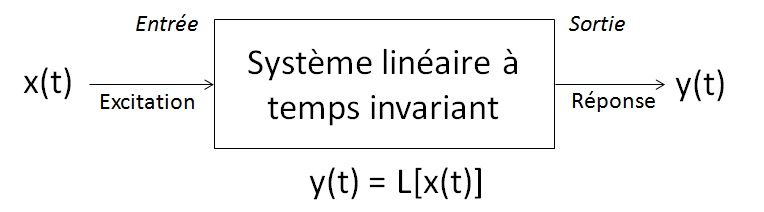
\includegraphics[scale=0.5]{images/LTI.jpg} 
		\caption{Représentation d'un système LTI comme une boîte noire reliant les signaux d'entrée et de sortie par un opérateur linéaire}	
		\label{Fig:LTI}
	\end{figure}
	
	Dans ce cours, L'étude des systèmes consiste prédire leur réponse à une excitation donnée, ou retrouver le signal d'entrée à partir de la sortie. 
	
	Nous présenterons dans ce cours des concepts et outils mathématiques qui permettront l'étude des signaux et systèmes linéaires (leur réponse), indépendamment de leur nature. Ils s'appliqueront aussi bien à des systèmes électroniques, mécaniques ou ???, tant que ceux-ci sont linéaires. Ce sera la même chose pour les signaux. Quelle que soit la nature des signaux, tant que ceux-ci seront continus, les concepts que nous présenterons resteront valables.
	
	
	\section{Les outil	
	
\chapter{Systèmes linéaires à temps invariant}
	Le but de ce chapitre est de présenter les concepts de base indispensables à l'étude des systèmes linéaires à temps invariants (LTI) et des signaux.
	Après une définition des critères qui caractérisent un système LTI, nous chercherons à répondre à la question suivante :
	comment déterminer efficacement la réponse d'un système linéaire lorsqu'il est soumis à une excitation quelconque ? Par efficacement, nous entendons :
	\begin{itemize}
		\item méthode mathématiquement "simple"
		\item méthode indépendante de l'excitation et des propriétés du système LTI
	\end{itemize}
	
	
	Pour cela, nous allons commencer par nous interroger sur la manière de représenter l'interaction entre l'entrée et la sortie d'un système, puis sur les notions d'excitation et de réponse. Nous distinguerons les notions de réponses naturelles et forcées, avant d'identifier deux familles d'excitation adaptées à l'étude des systèmes. Nous introduirons ensuite la notion de fréquence (complexe), qui nous offrira la possibilité d'étudier les signaux temporels dans le domaine fréquentiel,	ainsi que la notion de fonction de transfert qui facilitera l'étude des systèmes.
	
	
	\section{Définition d'un système LTI}

	\subsection{Linéarité} 
	Un système relie les signaux de sortie avec ceux d'entrée à l'aide d'un opérateur mathématique quelconque noté L.
	\begin{equation}\label{key}
	y(t) = L[x(t)] 
	\end{equation}
		
	Si L est un opérateur linéaire, alors le système est linéaire. On le vérifie s'il respecte la condition suivante : 
	
	Soit $y_{1}$ la réponse du système à une excitation donnée $x_{1}$. Soit $y_{2}$ la réponse du système à une excitation donnée $x_{2}$. Si le système est linéaire, alors la réponse y à une excitation x correspondante à la somme pondérée des excitations x1 et x2 sera la somme des réponses y1 et y2 pondérée de la même manière (équation \ref{def_linearite}), où a et b sont deux constantes.
	\begin{equation}\label{def_linearite}
	si    \left \{
	\begin{array}{l}
	x_{1}(t)\rightarrow y_{1}(t)  \\
	x_{2}(t)\rightarrow y_{2}(t)   \\
	\end{array}
	\right . alors: ax_{1}(t)+bx_{2}(t)\rightarrow ay_{1}(t)+by_{2}(t)
	\end{equation}
	
	
	Une des conséquences de la linéarité est la possibilité d'appliquer le principe de superposition.
	
	Les trois opérateurs linéaires de base que nous considérons dans l'étude des systèmes linéaires sont :
	\begin{itemize}
		\item proportionnel : $y = a\cdot x$ où a est une constante 
		\item intégration : $y = a\cdot \int f(x) \deriv x $ où a est une constante
		\item dérivée : $y = a\cdot \frac{df(x)}{dx} $ où a est une constante
	\end{itemize}
	On peut aisément vérifier qu'il respecte la condition \ref{def_linearite}.
	
	\subsection{Invariance temporelle}
	La condition d'invariance temporelle ou de stationnarité est respectée si la propriété suivante est vérifiée :
	\begin{equation}
	L[x(t-t_{0}]) = y(t-t_{0})]   ~~\forall t_{0} \in \mathbb{R}
	\end{equation}
	En d'autres termes, la réponse du système ne dépend pas de l'origine des temps choisie.
	
	\vspace{1\baselineskip}
	\underline{Exemple :}
	\vspace{0.5\baselineskip}
	

	
	L'effet du système sur le signal d'entrée peut s'écrire à l'aide de la fonction : $y(t)=2\frac{dx}{dt}$.
	Vérifions d'abord que cet opérateur est linéaire. Soit $ x_{1}(t)\rightarrow y_{}(t)=2\frac{dx_{1}}{dt}$ et  $ x_{2}(t)\rightarrow y_{2}(t)=2\frac{dx_{2}}{dt}$. L'entrée $x_{3}(t)=a\cdot x_{1}(t)+b\cdot x_{2}(t) $ avec a et b deux constantes quelconques donne le signal de sortie $y_{3}(t)$ définie par :
	\begin{equation*}
	y_{3}(t)=2\frac{dx_{3}}{dt}=2\frac{d}{dt}(a\cdot x_{1}(t)+b\cdot x_{2}(t))
	\end{equation*}
	\begin{equation*}
	y_{3}(t)=2a\frac{dx_{1}}{dt}+2b\frac{dx_{2}}{dt}
	\end{equation*}
	\begin{equation*}
	y_{3}(t)=ay_{1}(t)+by_{2}(t)
	\end{equation*}
	Le système est donc linéaire. Vérifions son invariance temporelle :
	\begin{equation*}
	x(t-t_{0}) \rightarrow 2\frac{d}{dt}x(t-t_{0})=y(t-t_{0})
	\end{equation*}
	
	
	\subsection{Passivité}
	Dans ce cours, on considèrera aussi des systèmes passifs, dans le sens où il n'y a pas d'énergie emmagasinée ou fournie par une entrée autre que celle sur laquelle on applique le signal d'entrée étudié.
	\subsection{Causalité}
	L'étude des systèmes linéaires passent par l'étude et la synthèse de fonctions mathématiques. Tous les systèmes linéaires physiquement réalisables peuvent être décrits par une fonction mathématique linéaire. Par contre, l'inverse n'est pas vraie : un système décrit par une fonction linéaire n'est pas nécessairement physiquement réalisable. Une caractéristique importante qui permet de différencier les systèmes physiquement réalisables de ceux qui ne le sont pas est la notion de causalité. On entend par physiquement réalisable un système pouvant "traiter" en temps réel les signaux d'entrée.
	Dans un système causal, l'effet ne peut pas précéder la cause (\ref{def_causal}). Un système sera physiquement réalisable s'il est causal, c'est-à-dire que sa réponse d'un système ne dépend que des états présents et passés de l'excitation.
	
	\begin{equation}\label{def_causal}
	\forall t < t_{0} : x(t) = 0 \rightarrow \forall t < t_{0} : y(t) = 0
	\end{equation}
	
	Les systèmes numériques peuvent être non causaux car ils sont capables de stocker les valeurs du signal d'entrée pour un traitement différé. On peut prendre l'exemple de l'application de floutage d'une image numérique. Celle-ci correspond à une matrice de données, représentant chaque pixel de l'image. Le floutage consiste à appliquer un filtre (par exemple gaussien) qui sera centré sur chaque pixel. Ce filtre effectue une somme pondérée du pixel central mais aussi des pixels voisins, situés avant et après le pixel central. L'effet du floutage d'un pixel dépend donc de pixels situés après dans l'ordre de rangement des pixels. 

	
	
	\section{Equation générale d'un système linéaire}
	La réponse d'un système linéaire sera gouvernée par trois types d'effet, pouvant se superposer : proportionnel, différenciateur et intégrateur. Globalement, un système linéaire est gouverné par une équation différentielle ordinaire donnée par \ref{equation_generale_LTI}. On l'appelle l'équation générale du système. Pour une excitation x(t) donnée, sa résolution permettra de déterminer la réponse y(t).
	
	\begin{equation}\label{equation_generale_LTI}
	\sum_{i=0}^M a_{i}\times \frac{d^{i}y}{dt^{i}} = \sum_{j=0}^N b_{j}\times \frac{d^{j}x}{dt^{j}}
	\end{equation}
	
	
	\section{Réponse d'un système}
	La réponse d'un système correspond au signal (ou aux signaux) de sortie de celui-ci lorsqu'il est excité par un (ou plusieurs) signal d'entrée. En reprenant l'équation générale \ref{equation_generale_LTI}, on remarque que l'on peut distinguer :
	\begin{itemize}
		\item la réponse propre ou naturelle d'un système, notée $y_{0}(t)$, correspondant à la solution de l'équation différentielle pour une excitation nulle.
		\item la réponse forcée, notée $y_{f}(t)$ correspondant à la solution de l'équation différentielle pour une excitation particulière x(t).
	\end{itemize}
	
	La réponse d'un système sera la superposition de ces deux réponses (hormis si le système n'est pas excité, auquel cas il n'y aura pas de réponse forcée).
	
	\begin{equation}
	y(t) = y_{0}(t)+y_{f}(t)
	\end{equation}
	
	Dans la suite du cours, nous ne nous intéresserons qu'à des systèmes causaux,  et nous considérerons que les excitations sont nulles pour t > 0.
	
	\section{Réponse naturelle d'un système LTI}
	Il s'agit de la partie de la réponse indépendante de l'excitation. Elle est donc intrinsèque aux caractéristiques du système. Elle se détermine en résolvant l'équation différentielle \ref{equation_generale_LTI} dans le cas où l'excitation x(t) est nulle.
	\begin{equation}\label{equa_diff_reponse_naturelle}
	\sum_{i=0}^M a_{i}\times \frac{d^{i}y}{dt^{i}} = 0
	\end{equation}
	On pourrait s'interroger sur le sens de cette réponse. Si le système n'avait pas emmagasiné d'énergie au départ, la réponse serait nulle, ce qui ne présente pas d'intérêt pour l'étude des systèmes. La réponse naturelle va donc s'observer sur un système que l'on a préalablement excité avant t = 0.  
	
	Comme l'excitation disparait pour t > 0, la réponse sera forcément transitoire. Seule une fonction présentant la même forme avant/après dérivation plusieurs fois peut être solution de l'équation \ref{equa_diff_reponse_naturelle}. Il n'existe qu'une seule forme de fonction avec une telle propriété : la forme exponentielle complexe (\ref{expo_complexe}).
	\begin{equation}\label{expo_complexe}
	y_{0}(t) = A \cdot exp(p t)       
	\end{equation}
	avec A et p $\in \mathbb{C}$.La forme générale de la réponse naturelle sera donc donnée par $ \sum_{i=0}^M a_{i}\cdot p^{i} \cdot exp(p \cdot t) $. Hormis la solution triviale $y_{0}(t) = 0$, la solution ce cette équation est donnée par \ref{solution_reponse_naturelle}.
	\begin{equation} \label{solution_reponse_naturelle}
	\sum_{i=0}^M a_{i}\cdot p^{i} = 0 \Rightarrow \prod_{i=1}^{M} (p-p_{i}) = 0     
	\end{equation}	
	Ce polynôme est appelée l'équation caractéristique du système. En effet, les caractéristiques de la réponse naturelle du système sont liées aux M solutions ou racines $p_{i}$ de cette équation. La réponse naturelle peut donc s'écrire sous la forme suivante :
	\begin{equation}\label{reponse_naturelle}
	y_{0}(t) = \sum_{i=1}^M A_{i}\cdot exp(p_{i} \cdot t) 
	\end{equation}
	où les termes $A_{i}$ dépendent des conditions initiales connues en un temps $ t_{0}$.
	
	\subsection{Fréquences naturelles d'un système LTI}
	Les M racines de l'équation caractéristique du systèmes sont appelées les fréquences naturelles ou propres. Elles sont complexes et de la forme suivante :
	\begin{equation}\label{freq_propre}
	p_{i} = \sigma_{i} + j\omega_{i} 
	\end{equation}	
	En reprenant \ref{reponse_naturelle}, la réponse naturelle pourra s'exprimer :
		
	\begin{equation}\label{Reponse_Naturelle}
	y_{0}(t) = \sum_{i=1}^M A_{i}exp(\sigma_{i}  t) exp(j\omega_{i} t)
	\end{equation}
	$\omega_{i}$ caractérise la pulsation de la réponse associée à cette racine, tandis que la partie réelle $\sigma_{i}$ indique l'atténuation ou l'amortissement de cette réponse. Leur connaissance est indispensable car ce sont elles qui caractérisent la forme temporelle de la réponse du système. La compréhension de l'évolution temporelle de la réponse du système va passer par l'analyse de ces racines. 
	
	\subsection{Plan p}
	Puisque les racines de l'équation caractéristique déterminent la réponse naturelle d'un système, il est intéressant d'établir un système de représentation graphique facilitant l'analyse du système. C'est le but de la représentation appelée plan complexe ou plan P , illustré à la figure \ref{Fig:Plan_P}. Il s'agit d'un repère cartésien dans lequel les racines sont placées, permettant de visualiser leurs parties réelles et imaginaires. Selon le positionnement des racines dans le plan P, les caractéristiques du système seront différentes, notamment la stabilité.
	\begin{figure}[h!]
		\centering
		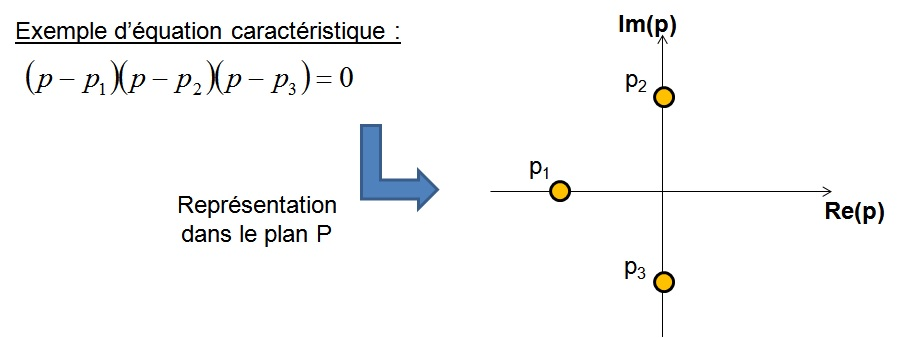
\includegraphics[scale=0.5]{images/Plan_P.jpg} 
		\caption{Placement des racines de l'équation caractéristique dans le plan P}	
		\label{Fig:Plan_P}
	\end{figure}

	\subsection{Analyse du plan p - Stabilité du système}
	La stabilité d'un système est une notion qui sera abordée plus en détail dans les cours d'automatique. Dans ce cours, nous utiliserons une définition au sens large : on entend par stabilité le fait que la réponse d'un système converge vers une valeur finie quelle que soit l'excitation appliquée (à condition que cette excitation converge). Dès que l'on conçoit un système, c'est une propriété indispensable qui doit être vérifiée.
	Un système est stable si et seulement si à toute entrée bornée, il fait correspondre une sortie bornée :
	\begin{equation}
	(\forall t \in \mathbb{R})~(|x(t)| \leq A),~avec~A \in \mathbb{R} \Rightarrow (|y(t)| \leq B),~avec~B \in \mathbb{R}
	\end{equation}
	
	
	La position des racines de l'équation caractéristique détermine à la fois la stabilité du système linéaire, mais aussi la forme temporelle de réponse. Pour l'admettre, considérons les cinq cas suivants, correspondant à cinq positions différentes d'une racine $p_{i}$ dans le plan P, et déterminons le type de réponse temporelle. On considère t > 0 :
	
	
	\begin{enumerate}
		\item $p_{i}$ est purement complexe ($\sigma_{i}$ = 0) : elle est située sur l'axe des ordonnées du plan P. La réponse  naturelle sera donc un signal purement (co)sinusoïdale, dont l'oscillation aura une fréquence ou une pulsation déterminée par $\omega_{i}$. Le système est en limite de stabilité car sa réponse oscille en permanence autour d'une valeur.
		\item $p_{i}$ est purement réel et négatif ($ \sigma $\textsubscript{i} \textless{} 0 et 		$ \omega $\textsubscript{i} = 0) : la racine est située sur l'axe des abscisses à 		gauche de l'origine. La réponse est une fonction exponentielle 		décroissante, sans la moindre oscillation, indiquant un complètement 		amorti. La réponse naturelle indique un système parfaitement stable.
		\item $p_{i}$ est purement réel et positif ($ \sigma $\textsubscript{i} \textgreater{} 0 et $ \omega $\textsubscript{i} = 0) : la racine est située sur l'axe des abscisses à droite de l'origine. La réponse est une fonction exponentielle croissante, sans la moindre oscillation, indiquant un complètement divergeant. La réponse naturelle indique un système instable.
		\item $p_{i}$ est une valeur complexe quelconque dont la partie réelle est négative ($ \sigma $\textsubscript{i} \textless{} 0 et  $ \sigma_{i} \neq 0 $) : la racine 	est située dans le demi plan à gauche de l'axe es ordonnées. La réponse va présenter une oscillation dont la fréquence est déterminée par $ \omega_{i}$, mais dans l'amplitude s'atténue plus ou moins rapidement au cours du temps selon la valeur  $ \sigma_{i} $. Cette réponse indique un système stable.
		\item $p_{i}$ est une valeur complexe quelconque dont la partie réelle est positive ($ \sigma $\textsubscript{i} \textgreater{} 0 et $ \omega_{i} \neq 0 $) : la racine est située dans le demi plan à droite de l'axe es ordonnées. La réponse va présenter une oscillation dont la fréquence est déterminée par $ \omega_{i} $, mais dans l'amplitude s'accroit plus ou moins rapidement au cours du temps selon la valeur  $ \sigma_{i} $. Cette réponse indique	un système instable.
		

	\end{enumerate}
	
	La figure ci-dessous illustre les types de réponse naturelle associée à une fréquence naturelle, selon sa position dans le plan P.
	\begin{figure}[h!]
		\centering
		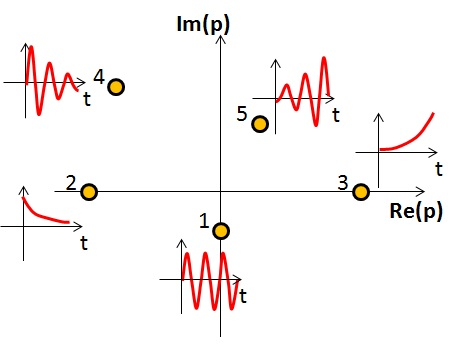
\includegraphics[scale=0.5]{images/reponse_vs_p.jpg} 
		\caption{Types de réponse naturelle en fonction de la position d'une racine dans le plan P.}	
		\label{Fig:reponse_vs_p}
	\end{figure}
	
	\underline{Remarque :} domaine fréquentiel
	
	On remarque que l'on est capable de représenter avec un point dans le
	plan p une fonction temporelle. Il s'agit de la même fonction, mais vue
	dans un autre domaine, que l'on appelle domaine fréquentiel. Dans ce domaine, la fonction n'est plus analysée à l'aide du temps, mais à l'aide de la fréquence. De manière générale, les fréquences sont des grandeurs complexes. Néanmoins, dans le cas de l'analyse des signaux, on considère uniquement des fréquences réelles.
	
	
	\subsection{Ordre d'un système linéaire}
	
	Plus l'équation caractéristique présente de racines, plus sa réponse
	devient complexe, puisqu'elle résulte de la superposition de plusieurs
	fréquences  comme le montre l'équation \ref{Reponse_Naturelle}. On appelle l'ordre
	d'un système le nombre de racines que présente son équation
	caractéristique. Il s'agit aussi de l'ordre ou du degré de l'équation
	différentielle caractérisant le système. Pour illustrer la notion
	d'ordre, nous allons analyser la réponse naturelle de deux systèmes
	électriques, caractérisés par des équations caractéristiques d'ordre 1 et 2. Vous retrouverez une analyse plus détaillée dans le cours d'électronique.
	
	\subsubsection{Exemple 1 : circuit RC}
		
	\begin{minipage}[l]{0.7\linewidth}
		On considère le circuit ci-contre, formée par une résistance R et un condensateur C. En t= 0, le condensateur est chargé, de sorte que la tension à ses bornes soit égale à $U_{C0}$. On note $U_{C}$ et $U_{R}$ les tensions aux bornes du condensateur et de la résistance. 	
	\end{minipage} \hfill
	\begin{minipage}[r]{0.4\linewidth}
		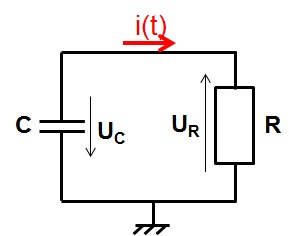
\includegraphics[scale=0.5]{images/circuit_RC_reponse_naturelle.jpg} 	
	\end{minipage}
	\vspace{0.5\baselineskip}
	On souhaite déterminer la réponse naturelle de ce circuit pour t > 0, sous la forme du courant électrique i(t) circulant au travers du circuit. On souhaite aussi déterminer la fréquence naturelle de ce circuit, caractérisant sa réponse transitoire.
	
	\vspace{1\baselineskip}
	Commençons par appliquer la loi des mailles à ce circuit, qui permet d'écrire : $U_{R}(t)+U_{C}(t)=0.$ En prenant en compte les relations tension-courant pour la résistance et le condensateur, cette relation peut être mise sous la forme ci-dessous ne faisant apparaître que le courant. Après différenciation de l'équation, on fait apparaître une équation différentielle du premier ordre. On constate que le terme RC est homogène à un temps. On l'appelle la constante de temps du circuit RC, généralement notée $\tau$.
	\begin{equation*}
	Ri(t)+\frac{1}{C}\int i(t) \deriv t=0~\rightarrow ~\frac{di}{dt}+\frac{1}{RC}i = 0
	\end{equation*}
	On retrouve une équation du même type que \ref{equa_diff_reponse_naturelle}. La solution de cette équation peut donc s'écrire : $i(t) = Ae^{pt}$, où A est lié aux conditions initiales et p est l'unique fréquence naturelle du système. En intégrant cette solution dans l'équation différentielle, on en déduit l'équation caractéristique de ce circuit (\ref{equa_carac_RC}).
	\begin{equation*}
	Ap\cdot e^{pt}+\frac{1}{RC} e^{pt}=0
	\end{equation*}
	\begin{equation}\label{equa_carac_RC}
	p+\frac{1}{RC}=p-p_{0}=0
	\end{equation}
	Cette équation présente une seule racine $p_{0} = -\frac{1}{RC}$. Ce circuit électrique est donc un système d'ordre 1. La racine est purement réelle et négative. Elle se situe donc à gauche de l'axe des imaginaires dans le plan P, traduisant le comportement stable et non oscillant du système (équivalent au point 2 de la figure \ref{Fig:reponse_vs_p}). La fréquence naturelle	indique donc une réponse naturelle du type exponentielle décroissante. Cela est confirmé par l'expression de la réponse naturelle du circuit, qui s'écrit :
	\begin{equation}\label{Reponse_naturelle_RC}
	i(t)=Aexp(p_{0}t)=Aexp(-\frac{t}{RC})~,~~t>0
	\end{equation}
	La valeur de A peut être déterminée à partir des conditions initiales en t = $0^{+}$. Le courant dans le circuit est alors donné par : $i(0)=\frac{U_{R}(0)}{R}=\frac{U_{C0}}{R}$. A partir de \ref{Reponse_naturelle_RC}, on en déduit $A=\frac{U_{C0}}{R}$.


	\subsubsection{Exemple 2 : circuit RLC}
	
	\begin{minipage}[l]{0.7\linewidth}
		On considère le circuit ci-contre, formée par une résistance R, un condensateur C et une bobine L montées en parallèle (R, L et C $geq$ 0). En t= 0, le condensateur est chargé, de sorte que la tension à ses bornes soit égale à $U_{C0}$. On note $i_{C}$, $i_{R}$ et $i_{L}$ les courants traversant ces trois composants. 	
	\end{minipage} \hfill
	\begin{minipage}[r]{0.4\linewidth}
		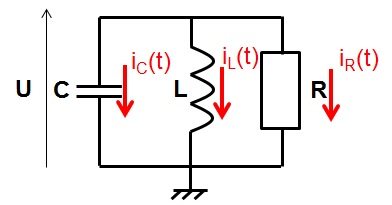
\includegraphics[scale=0.5]{images/circuit_RLC_reponse_naturelle.jpg} 	
	\end{minipage}
	\vspace{0.5\baselineskip}
	On souhaite déterminer la réponse naturelle de ce circuit pour t > 0, sous la forme de la tension u(t) circulant aux bornes du circuit. On souhaite aussi déterminer la fréquence naturelle de ce circuit, caractérisant sa réponse transitoire.

	\vspace{1\baselineskip}
	Commençons par appliquer la loi des nœuds à ce circuit, qui permet d'écrire : $i_{C}(t)+i_{R}(t)+i_{L}(t)=0.$ En prenant en compte les relations tension-courant pour la résistance et le condensateur, cette relation peut être mise sous la forme ci-dessous ne faisant apparaître que le courant. Après différenciation de l'équation, on fait apparaître une équation différentielle du second ordre. Pour simplifier les notations, on pose : $\alpha = \frac{1}{2RC} $ et $\omega^{2} = \frac{1}{LC}$.
	\begin{equation*}
	C\frac{du}{dt}+\frac{u(t)}{R}+\frac{1}{L}\int u(t) \deriv t=0~\rightarrow ~\frac{d^{2}u}{dt^{2}}+\frac{1}{RC}\frac{du}{dt}+\frac{1}{LC}u(t) = 0
	\end{equation*}
	\begin{equation*}
	\frac{d^{2}u}{dt^{2}}+2\alpha \frac{du}{dt}+\omega^{2}u(t) = 0
	\end{equation*}
	
	On retrouve une équation du même type que \ref{equa_diff_reponse_naturelle}. La solution de cette équation peut donc s'écrire : $u(t) = Ae^{pt}$. En intégrant cette solution dans l'équation différentielle, on en déduit l'équation caractéristique de ce circuit (\ref{equa_carac_RLC}).
	\begin{equation*}
	(p^{2}+2\alpha p+\omega^{2})Ae^{pt}=0 
	\end{equation*}
	\begin{equation}\label{equa_carac_RLC}
	p^{2}+2\alpha p+\omega^{2}=(p+p_{1})(p+p_{2})=0
	\end{equation}
	Cette équation présente deux racines $p_{1}$ et $p_{2}$. Ce circuit électrique est donc un système d'ordre 2, dont la réponse naturelle va s'écrire :
	\begin{equation}\label{key}
	u(t) = A_{1}e^{p_{1}t}+A_{2}e^{p_{2}t}
	\end{equation}
	
	 où $A_{1}$ et $A_{2}$ dépendent des conditions initiales. Selon la valeur de R, L et C, la nature et la position de ces racines dans le plan P va changer, modifiant le comportement transitoire du circuit. Pour déterminer ces racines, il suffit de résoudre une équation d'ordre 2, dont le déterminant est donné par : $\Delta = 4(\alpha^{2}-\omega^{2})$. La nature des racines varie selon le signe du déterminant :
	\begin{equation}
	si~\alpha \geq \omega : \left \{
		\begin{array}{l}
			p_{1}=\frac{-2\alpha +\sqrt{\Delta}}{2}=-\alpha+\sqrt{\alpha^{2}-\omega^{2}} \\
			p_{2}=\frac{-2\alpha -\sqrt{\Delta}}{2}=-\alpha-\sqrt{\alpha^{2}-\omega^{2}} \\
		\end{array}
	\right.
	\end{equation}
	\begin{equation}
	si~\alpha < \omega : \left \{
	\begin{array}{l}
	p_{1}=\frac{-2\alpha +j\sqrt{-\Delta}}{2}=-\alpha+j\sqrt{\omega^{2}-\alpha^{2}} \\
	p_{2}=\frac{-2\alpha -j\sqrt{-\Delta}}{2}=-\alpha-j\sqrt{\omega^{2}-\alpha^{2}} \\
	\end{array}
	\right.
	\end{equation}
	On peut distinguer plusieurs types de comportement transitoire distincts selon les valeurs de $\alpha$ et $\omega$ :
	\begin{itemize}
		\item si $\alpha \neq 0$, alors les deux racines présentent une partie réelle négative. Le système présente donc un caractère stable.
		\item si $\alpha \geq \omega$, les deux racines sont purement réelles et négatives. Dans le plan P, elles sont situées sur l'axe des réels à gauche de l'axe des imaginaires. La réponse du circuit sera du type exponentiel décroissant sans oscillation (équivalent au point 2 de la figure \ref{Fig:reponse_vs_p}).
		\item si $\alpha < \omega$ et $\alpha neq 0$, les deux racines sont conjuguées. Elles sont situées à gauche de l'axe des imaginaires dans le plan P. La réponse du circuit sera du type oscillation amortie de pulsation $\sqrt{\omega^{2}-\alpha^{2}}$ (équivalent au point 4 de la figure \ref{Fig:reponse_vs_p}). 
		\item si $\alpha = 0$, les deux racines sont purement imaginaires et conjuguées. Elles sont placées sur l'axe imaginaire du plan P, symétriquement à l'axe de réels. La réponse du circuit sera une oscillation non amortie de pulsation $\omega$ (équivalent au point 1 de la figure \ref{Fig:reponse_vs_p}). 
	\end{itemize}
	\vspace{1\baselineskip}

	
	\section{Réponse forcée}
	
	La réponse forcée est la solution de l'équation générale du système pour une excitation non nulle. La réponse va dépendre de la forme de l'excitation, mais aussi des
	propriétés du système. Puisque la réponse dépend de l'excitation, il est
	préférable de déterminer des excitations dont les propriétés
	faciliteront l'analyse de la réponse forcée d'un système. Pour cela, il
	faut chercher des familles d'excitation dont la forme n'est pas modifiée
	par l'effet du système LTI. Ainsi, en connaissant la forme de
	l'excitation, on déduira immédiatement la forme de la réponse. Seuls
	quelques coefficients que nous préciserons seront à calculer.
	
	Nous allons nous intéresser à deux familles d'excitations répondant à ce critère : l'excitation
	exponentielle complexe (que nous avons rencontré précédemment) et la
	famille d'excitation impulsionnelle.
	
	\subsection{Excitation exponentielle complexe}
	L'excitation exponentielle complexe présente la forme suivante :
	
	\begin{equation}\label{exc_expo_complexe}
		x =    \left \{
		\begin{array}{l l}
		\hat{X} \cdot exp(p_{x}t)  & si~t>0 \\
		0   & sinon \\
		\end{array}
		\right .
	\end{equation}
	
	où $ \hat{X} = |X| \cdot exp(j \theta)$ est l'amplitude complexe ou le phaseur du signal (voir annexe A) et $ p_{x} = \alpha $+j$ \omega $ sa fréquence complexe. Dans le cas où l'on s'intéresse à des signaux réels (cas rencontré en pratique), elle peut s'écrire :
	\begin{equation}\label{exc_expo_complexe_reel}
	x(t) =    \left \{
	\begin{array}{l l}
	Re[\hat{X} \cdot e^{p_{x}t)}] = |X| \cdot e^{\alpha t} \cdot cos(\omega t+\theta)  & si~t>0 \\
	0   & sinon \\
	\end{array}
	\right .
	\end{equation}
	Comme dans le cas de la fréquence naturelle, la fréquence complexe peut
	être représentée dans le plan P. Sa position indique qualitativement la
	forme temporelle de l'excitation. Si p\textsubscript{x} est purement
	réelle, l'excitation est une fonction exponentielle pure. Si
	p\textsubscript{x} est purement complexe, l'excitation est une fonction
	cosinusïdale pure. L'excitation est dite monochromatique. |X| représente son amplitude et $\theta$ sa phase.
	
	\vspace{0.5\baselineskip}
	\underline{Exemple :}
	Récrivez les expressions des fonctions ci-dessous sous la forme de fonctions réelles : $y(t)=Re[(1+j)e^{(-2+j)t}]$ et $z(t) = Re[2e^{j\frac{\pi}{2}}e^{j10t}]$.
	
	Les deux fonctions sont des exponentielles complexes. Elles représentent des signaux temporels réels puisqu'on ne conserve que la partie réelle. Le phaseur de la fonction y(t) peut s'écrire $\hat{Y}=1+j=\sqrt{2}e^{j\frac{\pi}{4}}$. La fréquence complexe contient une partie réelle négative donnant un comportement d'exponentielle décroissante à l'amplitude, et une partie imaginaire donnant un comportement oscillant de pulsation égale à 1. La fonction y(t) peut donc s'écrire : $y(t)=\sqrt{2}e^{-2t}cos(t+\frac{\pi}{4})$.
	En procédant de même pour la fonction z(t), on remarque que sa fréquence est purement complexe. Il s'agit d'une fonction cosinusoïdale s'écrivant : $z(t)=2cos(10t+\frac{\pi}{2})$.
	
	\vspace{0.5\baselineskip}
	
	
	L'excitation exponentielle complexe a une propriété remarquable : l'action d'un opérateur linéaire (proportionnel, intégrateur ou différentiel) laisse sa forme inchangée. Seule son amplitude et sa localisation temporelle sont modifiées. On peut donc en déduire une propriété des systèmes LTI : lorsqu'un système linéaire est excité par un signal exponentiel complexe (en pratique, un signal sinusoïdal), la réponse sera aussi une fonction du même type et de même fréquence complexe. Seule l'amplitude et la phase changeront.
	
	
	
	\subsection{Familles d'excitations impulsionnelles}
	
	Nous parlons ici de familles car nous allons parler de plusieurs
	fonctions, reliées entre elles et associées à une excitation très importante
	dans l'analyse des systèmes et des signaux : l'impulsion de Dirac.
	
	\subsubsection{Echelon unitaire ou fonction de Heaviside}
	
	\begin{minipage}[l]{0.7\linewidth}
		L'échelon unitaire ou fonction de Heaviside est décrite sur la figure ci-contre et est décrite par l'équation \ref{Heaviside}. Elle représente le signal que l'on obtiendrait derrière un interrupteur
		idéal que l'on fermerait à $t = t_{0}$. Son expression est donnée par \ref{Heaviside}. Dans la suite, on utilisera principalement $t_{0} = 0$.	
	\end{minipage} \hfill
	\begin{minipage}[r]{0.4\linewidth}
		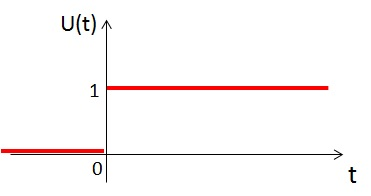
\includegraphics[scale=0.5]{images/Heaviside.jpg} 	
	\end{minipage}
	%\vspace{0.5\baselineskip}
	 
	\begin{equation}\label{Heaviside}
	u(t-t_{0}) = \left \{
	\begin{array}{l l}
	1  & si~t>t_{0} \\
	0   & sinon \\
	\end{array}
	\right .	 	
	\end{equation}
	
	
	Cette fonction peut être utilisée pour représenter n'importe quelle autre fonction avec une allure en marches d'escalier, comme l'illustre l'exemple présenté sur la figure \ref{Fig:Utilisation_Heaviside}. A partir de trois fonction de Heaviside dont les instants d'apparition de l'échelon sont décalés, il est possible de générer une forme d'onde plus complexe.
	\begin{figure}[h!]
		\centering
		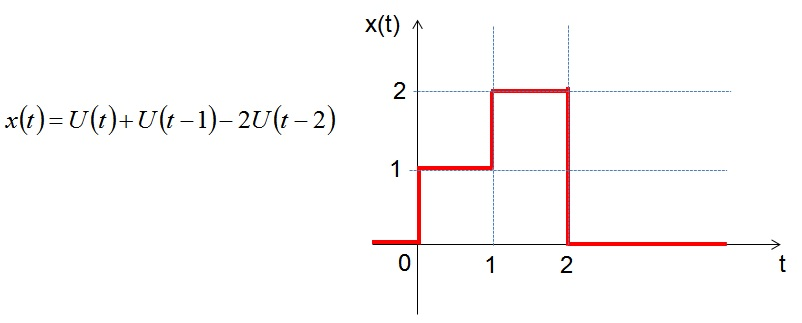
\includegraphics[scale=0.5]{images/Utilisation_Heaviside.jpg} 
		\caption{Exemple d'utilisation de la fonction de Heaviside pour bâtir une fonction plus complexe}	
		\label{Fig:Utilisation_Heaviside}
	\end{figure}
	
	La fonction de Heavisde peut servir de base pour générer d'autres fonctions, par intégration ou différenciation. Par exemple, en l'intégrant une fois, on obtient la fonction rampe. Si on l'intègre n fois, on peut obtient des fonctions présentant une croissance polynomiale en fonction du temps (\ref{integration_Heaviside}). 
	\begin{equation}\label{integration_Heaviside}
	u^{(-n)}(t) = \frac{t^{n}}{n!} \cdot u(t)	 	
	\end{equation}	
	Le cas de la dérivation est plus complexe car elle entraine l'apparition d'une discontinuité. En effet, la dérivée de la fonction de Heaviside devient infinie en $t_{0}$. Cet écueil ne peut se traiter qu'en utilisant la théorie des distributions, qui va permettre de définir l'impulsion de Dirac.
	
	\subsubsection{Impulsion ou distribution de Dirac}
	
	L'impulsion de Dirac se trouve en différenciant l'échelon unitaire (\ref{Dirac}). On
	voit immédiatement apparaître un problème : la dérivée est nulle sauf là
	où l'échelon présente une discontinuité. Sa dérivée devient infinie.
	L'impulsion de Dirac n'est pas une fonction au sens classique, mais une
	distribution. Voir annexe. 

	
	\begin{minipage}[l]{0.45\linewidth}
			Il est possible de donner une justification physique à l'impulsion de Dirac, comme illustré sur la figure ci-contre. On considère une fonction échelon avec un temps de transition finie $\tau$. En dérivant cette fonction, on obtient une fonction décrivant une impulsion brève de durée $\tau$. L'aire de cette fonction, associée à son énergie, est égale à 1. Au fur et à mesure que la durée $\tau$ décroit, l'amplitude de cette impulsion croit, mais son aire reste unitaire. Le passage à la limite montre que l'impulsion tend à devenir nulle partout, sauf à l'origine où l'amplitude deviendrait infinie. L'impulsion de Dirac est donc une abstraction mathématique permettant de définir une impulsion infiniment courte.	
	\end{minipage} \hfill
	\begin{minipage}[r]{0.55\linewidth}
		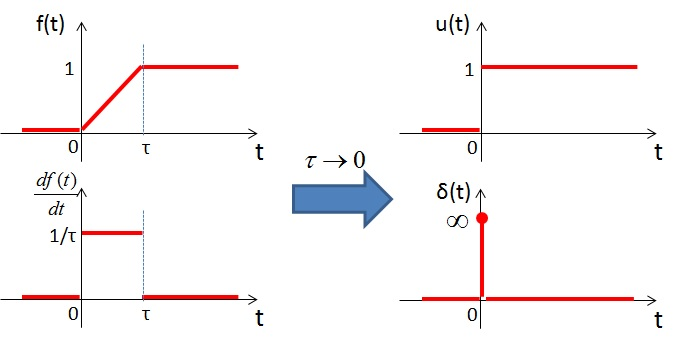
\includegraphics[scale=0.5]{images/generation_Dirac.jpg} 	
	\end{minipage}
	\vspace{0.5\baselineskip}
	
	
	\begin{equation}\label{Dirac}
	\delta (t) = \frac{du(t)}{dt}	 	
	\end{equation}
	
	La distribution de Dirac présente une propriété intéressante pour l'étude des signaux : la propriété d'échantillonnage, donnée par \ref{Dirac_echantillonage_1} et \ref{Dirac_echantillonage_2}. Elle permet de "collecter" un point unique en un temps  $t_{0}$ sur une fonction quelconque.
	\begin{equation}\label{Dirac_echantillonage_1}
	\int_{-\infty}^{+\infty} \delta (t) \cdot f(t) \deriv t = f(0) 	 
	\end{equation}
	\begin{equation}\label{Dirac_echantillonage_2} 	
	\int_{-\infty}^{+\infty} \delta (t-t_{0}) \cdot f(t) \deriv t = f(t_{0}) 
	\end{equation}
	
	\vspace{0.5\baselineskip}
	Revenons au problème initial de sélection de familles d'excitation inchangées par l'effet d'un système LTI. On peut remarquer que cette propriété est aussi vérifiée avec la famille d'excitation impulsionnelle. L'action d'un opérateur proportionnel, intégrateur ou dérivée appliquée à une fonction de cette famille donnera une nouvelle fonction appartenant aussi à cette famille.
	
	
	\section{Les différents types de réponse caractérisant les systèmes LTI}
	Maintenant que nous avons défini deux familles d'excitation adaptées à l'étude des systèmes LTI, nous pouvons définir plusieurs types de réponse qui nous aideront à analyser les propriétés de ces systèmes.
	\subsection{Réponse indicielle}
	Elle correspond à la réponse d'un système excité par une fonction de Heavisde. On la note a(t).
	\begin{equation}\label{key}
	si~x(t)=u(t)~\rightarrow ~y_{f}(t)=a(t)
	\end{equation}
	
	
	Cas d'un système d'ordre 1 : Exo corrigé ou TD
	
	Cas d'un système d'ordre 2 : Exo corrigé ou TD
	
	
	\subsection{Réponse impulsionnelle}
	Elle correspond à la réponse d'un système excité par une impulsion de Dirac, que l'on note h(t). Même si l'amplitude de cette impulsion est infinie, son énergie vaut 1. Au lieu de représenter cette valeur infinie, nous utiliserons la valeur de 1. N'oublions pas qu'il ne s'agit pas d'une fonction mais d'une distribution, qui n'a du sens qu'à l'intérieur d'une intégrale.
	\begin{equation}\label{key}
	si~x(t)=\delta (t)~\rightarrow ~y_{f}(t)=h(t)
	\end{equation}
	Quel que soit le système LTI considéré, puisque l'excitation devient nulle pour t > 0, on retrouve le calcul de la réponse naturelle. L'application de l'impulsion en t=0 ne fait que changer les conditions initiales.
	
	\begin{equation}\label{}
	si~x(t)=\delta (t)~\rightarrow ~y_{f}(t) = y_{0}(t)	 	
	\end{equation}
	
	\underline{Remarque : autre manière de déterminer la réponse impulsionnelle}
	
	Sans démonstration, on peut affirmer que si on différencie l'excitation, on peut déterminer la nouvelle réponse en différenciant la réponse à l'excitation initiale : si $y(t) = L[x(t)]$ alors $\frac{dy}{dt} = L[\frac{dx}{dt}] $.
	Ainsi, puisque l'impulsion de Dirac est la dérivée de l'échelon unitaire, si on connait la réponse indicielle, on peut retrouver la réponse impulsionnelle en dérivant la réponse indicielle.
	
	\vspace{1\baselineskip}
	La réponse impulsionnelle va nous fournir un moyen de calculer la
	réponse d'un système LTI à n'importe quelle excitation, en effectuant
	les calculs uniquement dans le domaine temporel. C'est ce que nous
	allons démontrer. Tout signal peut être vu comme une somme infinie
	d'impulsion de Dirac, pondérée et décalée dans le temps. Comme le montre
	la figure \ref{Fig:Approx_excitation_Dirac}, une excitation quelconque x(t) peut être
	approximée par une suite de rectangles adjacents, de largeur $ \Delta \tau $, que
	l'on peut remplacer par des impulsions de Dirac équivalentes de même
	surface. Ainsi, elles transportent la même énergie. Si la largeur $ \Delta \tau $
	tend vers zéro, cette approximation devient de plus en plus juste. Dans
	l'exemple considéré, on suppose que x(t) = 0 pour t \textless{} 0 par
	souci de lisibilité. Le même raisonnement resterait juste avec x(t) non
	nul pour t \textless{} 0. L'excitation peut alors s'approximer par :
	
	
	\begin{equation*}\label{}
	\sum_{n=-\infty}^{+\infty}x(n\Delta \tau) \cdot	\Delta \tau \cdot \delta (t-n\Delta \tau)	
	\end{equation*}
	
	\begin{figure}[h!]
		\centering
		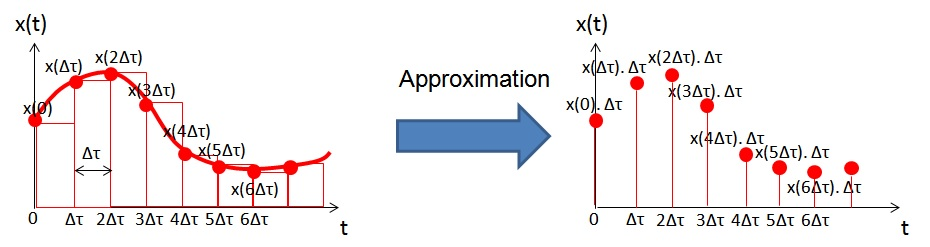
\includegraphics[scale=0.5]{images/Approx_excitation_Dirac.jpg} 
		\caption{Excitation quelconque x(t) approximée par une suite d'impulsion de Dirac}	
		\label{Fig:Approx_excitation_Dirac}
	\end{figure}
	Supposons que cette excitation attaque l'entrée d'un système LTI dont la réponse impulsionnelle h(t) est connue (Fig. \ref{Fig:reponse_impuls_illustration}). Par souci de lisibilité, on suppose aussi que h(t) = 0 pour t < 0.
	\begin{figure}[h!]
		\centering
		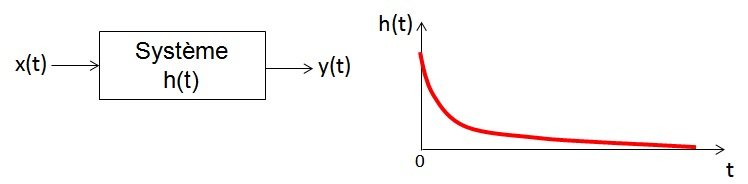
\includegraphics[scale=0.5]{images/reponse_impuls_illustration.jpg} 
		\caption{Réponse impulsionnelle d'un système}	
		\label{Fig:reponse_impuls_illustration}
	\end{figure}	
	
	Chaque impulsion élémentaire composant x(t) et apparaissant à l'instant
	$ k \times \Delta \tau $ contribue à la réponse en sortie, comme l'illustre la figure \ref{Fig:illustration_reponse_impuls_2}. Chacune d'entre elles produit une réponse égale à la réponse impulsionnelle du système, mais :
	
	\begin{itemize}
		\item pondérée par l'amplitude de l'excitation d'entrée à l'instant $ k \times \Delta \tau $
	
		\item décalée dans le temps de $ k \times \Delta \tau $~
	\end{itemize}
	\begin{figure}[h!]
		\centering
		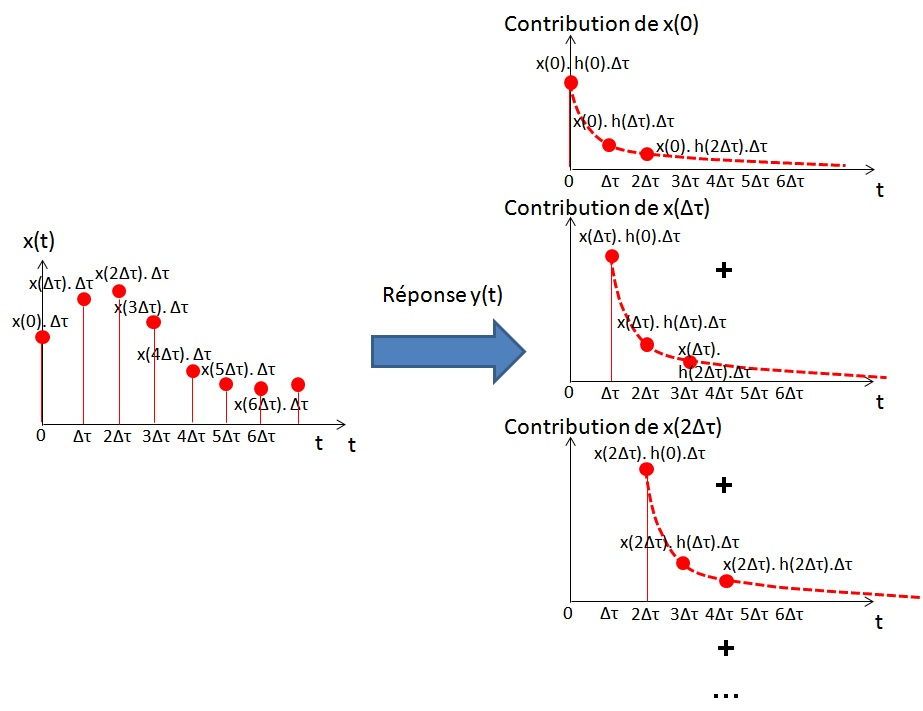
\includegraphics[scale=0.5]{images/illustration_reponse_impuls.jpg} 
	\end{figure}
	\begin{figure}[h!]
		\centering
		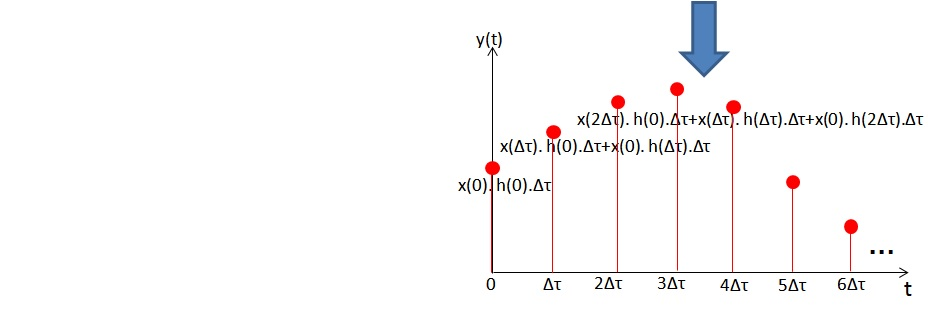
\includegraphics[scale=0.6]{images/illustration_reponse_impuls_2.jpg}
		\caption{Construction de la réponse impulsionnelle}	
		\label{Fig:illustration_reponse_impuls_2} 
	\end{figure}

	La réponse globale du système est obtenue en sommant l'ensemble des contributions de chaque impulsion élémentaire formant l'excitation. Elle peut alors s'approximer par : 
	\begin{equation*}\label{key}
	\sum_{n=-\infty}^{+\infty} x(n\Delta \tau) \cdot \Delta \tau \cdot h(t-n\Delta \tau)
	\end{equation*}
	
	En faisant tendre $ \Delta \tau $ vers zéro, cette somme converge vers une intégrale
	donnée par la relation ci-dessous. Ce calcul intégral particulier,
	faisant intervenir le produit de deux fonctions dont les indices $\tau $ et
	t-$\tau $ sont balayés dans des directions opposées, porte un nom : le produit
	de convolution. Cette opération est symbolisée par le signe *.
	\begin{equation}\label{Demo_produit_convolution}
	y(t) = \lim_{\Delta t \to 0} \sum_{n=-\infty}^{+\infty} x(n\Delta t) \cdot \Delta t \cdot h(t-n\Delta t) = \int_{-\infty}^{+\infty} x(\tau) \cdot h(t-\tau) \deriv \tau = x*h(t)
	\end{equation}
	
	Cette relation basée sur le produit de convolution fournit donc un outil de calcul de la réponse du système directement dans le domaine temporel. Cependant, c'est un calcul complexe, passant par une opération longue et fastidieuse si elle est effectuée à la main. Nous y reviendrons dans le chapitre 7, qui sera consacré au calcul des réponses des systèmes LTI directement dans le domaine temporel. Cependant, avant d'aborder ce point, nous allons d'abord considérer le cas d'une excitation exponentielle complexe pour dériver le concept de fonction de transfert défini dans le domaine fréquentiel. Nous verrons que dans ce domaine, le calcul de la réponse du système est beaucoup plus aisée !
	
	\subsubsection{Condition pour garantir la causalité}
	Un système est causal si sa réponse ne dépend que des états passés et présents. A partir de la réponse impulsionnelle, on peut en déduire une condition : il faut que h(t) = 0 pour t < 0. Les systèmes causaux sont les seuls à être physiquement réalisables. Le calcul de la réponse d'un système causal à partir de sa réponse impulsionnelle peut s'écrire :
	\begin{equation}\label{}
	y(t) = \int_{0}^{+ \infty} x(\tau) \cdot h(t-\tau)d\tau = x*h(t)
	\end{equation}
	\vspace{1\baselineskip}	
	
	
	\subsection{Réponse à une exponentielle complexe - Fonction de transfert}
	On considère une excitation exponentielle complexe. La réponse forcée a donc la même forme que l'excitation, et présente la même fréquence complexe. La seule inconnue est le phaseur $\hat{Y}$ de la réponse. Soit l'excitation $ x(t) = Re[\hat{X} \cdot e^{pt}]$ et la réponse $ y_{f}(t) = Re[\hat{Y} \cdot e^{pt}]$ pour t > 0. Si on reprend l'équation différentielle ordinaire générale d'un système LTI donnée par \ref{equation_generale_LTI}, on peut écrire la relation suivante.
	
	\begin{equation*}\label{}
	\sum a_{i} \cdot Re[p^{i} \cdot \hat{Y} \cdot exp(pt)] = \sum b_{i} \cdot Re[p^{j} \cdot \hat{X} \cdot exp(pt)]
	\end{equation*}
	\begin{equation*}\label{}
	\sum a_{i} \cdot Re[p^{i} \cdot \hat{Y}] = \sum b_{i} \cdot Re[p^{j} \cdot \hat{X}]
	\end{equation*}
	\begin{equation*}\label{}
	\hat{Y} \cdot \sum a_{i} \cdot Re[p^{i}] = \hat{X} \cdot \sum b_{i} \cdot Re[p^{j}]
	\end{equation*}
	
	On peut donc facilement déterminer le phaseur $\hat{Y}$ associée à la réponse, c'est-à-dire le module et le déphasage de la réponse. 
	On peut alors caractériser l'effet du système à une excitation exponentielle complexe quelconque sous une forme appelée fonction de transfert, définie comme le rapport entre les phaseurs de réponse et d'excitation, et défini pour toutes les fréquences complexes. 
	\begin{equation}\label{Def_fonction_tranfert}
	H(p) = \frac{Y}{X} (p) = \frac{\hat Y}{\hat X} (p)= \frac{\sum a_{i} \cdot Re[p^{i}]}{\sum b_{i} \cdot Re[p^{j}]}=G\frac{\prod_{i=1}^{M} (p-p_{i})}{\prod_{j=1}^{N} (p-p_{j})}
	\end{equation}
	De manière générale, l'équation \ref{Def_fonction_tranfert} peut s'écrire comme une fraction rationnelle entre deux polynômes, où G est un terme constant. Les N racines du dénominateur sont les pôles de la fonction de transfert et les M racines du numérateur sont appelées les zéros de la fonction de transfert. Comme leur nom l'indique, ils annulent la fonction de transfert lorsque la fréquence $p=p_{j}$. Les pôles sont les mêmes que ceux identifiés dans la réponse naturelle ! Ils ont un rôle prépondérant sur la stabilité du système et la nature de la réponse. Les outils permettant d'étudier l'influence des pôles et des zéros sur la réponse d'un système sortent du cadre de ce cours et seront abordés dans vos cours d'automatique.\\
	
	Avec une excitation exponentielle complexe, l'action du système LTI peut donc se résumer à la multiplication de l'excitation par la fonction de transfert.
	On peut souligner la facilité de la méthode. Une fois la fonction de transfert connue à une fréquence complexe donnée, la réponse forcée à une exponentielle complexe de même fréquence est trouvée en multipliant le phaseur d'entrée par la fonction de transfert (\ref{Relation_Entree_Sortie_Fonction_Transfert}).
	\begin{equation}\label{Relation_Entree_Sortie_Fonction_Transfert}
	\hat{Y}(p) = H(p)\cdot \hat{X}(p)=|H(p)||X(p)|e^{j(arg(H(p))+arg(\hat{X}(p)))}	
	\end{equation}
	
	\vspace{1\baselineskip}
	
	
	\underline{Réponse en fréquence en régime permanent :} 
	dans le cas général, l'excitation est complexe. Le cas particulier où $\sigma$ = 0 correspond au cas d'une dite monochromatique ou harmonique. On parlera alors de réponse en fréquence. Il correspond aussi au cas du régime permanent avec $\sigma$ < 0, c'est-à-dire que t devient suffisamment grand pour que l'influence du terme $e^{\sigma t}$ devienne négligeable. 
	La réponse du système se trouve facilement en remplaçant la fréquence complexe p par $j\omega$. En considérant une excitation cosinusoïdale d'amplitude égale à X et de phase $\Phi_{x}$, la réponse du système est donnée par la relation suivante.
	
	\begin{equation}\label{calcul_reponse_fonction_transfert}
	y(t) = Re[|H(\omega)|X\cdot e^{j(\omega t+arg(H(p))+\Phi_{x})}] =|H(\omega)|X\cdot cos(\omega t+arg(H(p))+\Phi_{x})
	\end{equation}
	
	La réponse est une grandeur complexe. Le module de la réponse en fréquence est le gain en amplitude de la fonction de transfert du système ou du filtre. Le déphasage du signal en sortie du filtre par rapport au signal d'entrée est l'argument de la fonction de transfert. Le module et la phase sont des fonctions de la pulsation $\omega$.
	
	
	\subsubsection{Exemple}
	
	\begin{minipage}[l]{0.7\linewidth}
		On reprend l'exemple du circuit RC abordé dans la partie IV.4. On considère toujours que le condensateur est chargé initialement en t = 0, avec une tension à ses bornes notée $U_C0$. Le circuit est excité par un signal délivrant une excitation exponentielle complexe $U_{E}(t)=Xe^{pt}$ avec t > 0 et X l'amplitude complexe. La réponse du circuit correspond à la tension mesurée aux bornes de la résistance R ou tension de sortie. Déterminez la fonction de transfert de ce circuit. Indiquez quels sont les pôles et les zéros. Quelle est la réponse à un signal cosinuoïdal, d'amplitude unitaire et de phase nulle ?	
	\end{minipage} \hfill
	\begin{minipage}[r]{0.4\linewidth}
		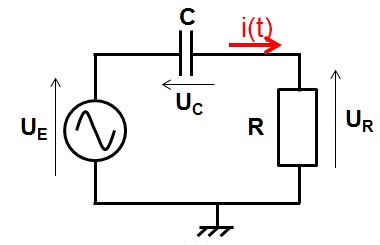
\includegraphics[scale=0.5]{images/circuit_RC_reponse_forcee.jpg} 	
	\end{minipage}
	\vspace{0.5\baselineskip}

	La réponse du circuit $U_{R}$ est la superposition de la réponse naturelle $U_{R0}$ et de la réponse forcée $U_{Rf}$. La réponse naturelle est liée à la présence d'une condition initiale : ici, le stockage d'une charge dans le condensateur à t=0. Sans charge initialement stockée, la réponse naturelle aurait été nulle. Nous avions établi la réponse naturelle de ce circuit en terme de courant. Nous pouvons aisément l'adapter pour la donner en terme de tension de sortie.
	\begin{equation*}\label{}
	U_{R0}(t)=Ri_{0}(t)=U_{C0}exp(-\frac{t}{RC})~,~~t>0
	\end{equation*}
	La réponse forcée est provoquée par l'excitation du circuit en t > 0, indépendamment de la présence d'une condition initiale. Commençons par établir une équation différentielle reliant la tension de sortie $U_{Rf}$ et l'excitation $U_{E}(t)$. On utilise la loi des mailles. Après une dérivation, on obtient l'équation \ref{equa_diff_reponse_forcee_RC}.
	\begin{equation*}\label{}
	U_{E}(t)=U_{C}(t)+U_{R}(t) ~ \Rightarrow ~ U_{E}(t)=\frac{1}{C}\int i(t) \deriv t+U_{R}(t)~ \Rightarrow ~U_{E}(t)=\frac{1}{RC}\int U_{R}(t) \deriv t+U_{R}(t)
	\end{equation*} 
	\begin{equation}\label{equa_diff_reponse_forcee_RC}
	\frac{dU_{E}}{dt}=\frac{U_{R}}{RC}+\frac{dU_{R}}{dt}
	\end{equation}
	L'excitation étant de type exponentielle complexe et le circuit linéaire, la réponse est aussi de type exponentielle complexe. Elle s'écrit : $U_{Rf}(t)=Ye^{pt}$. Replaçons les termes $U_{E}$ et $U_{R}$ par leurs expressions respectives dans \ref{equa_diff_reponse_forcee_RC} et exprimons le rapport entre ces deux grandeurs pour obtenir la fonction de transfert H(p) de ce circuit (équation \ref{TF_RC_forcee}).
	\begin{equation*}
	pXe^{pt}=\frac{1}{RC} Ye^{pt}+pYe^{pt} ~\Rightarrow~pU_{E}(t)=\frac{1}{RC}U_{Rf}(t)+pU_{Rf}(t)
	\end{equation*}
	\begin{equation}\label{TF_RC_forcee}
	H(p)=\frac{U_{Rf}}{U_{E}}(p)=\frac{1}{p+\frac{1}{RC}}
	\end{equation}

	La fonction de transfert du système ne présente aucun zéro et un seul pôle $p_{0}$, qui est exactement le même que celui identifié dans l'analyse de la réponse naturelle. Ce n'est pas une surprise car les pôles agissent sur la stabilité, qui est une caractéristique intrinsèque du système indépendante de l'excitation. Le pôle étant purement réel et négatif, on peut conclure que le système sera stable. On peut exprimer la fonction de transfert sous la forme module-phase :
	\begin{equation*}
	|H(p)|=\frac{1}{\sqrt{1+(\frac{p}{p_{0}})^{2}}}~~~~~Arg(H(p))=-atan(\frac{p}{p_{0}})
	\end{equation*}
	
	Calculons maintenant la réponse forcée à un signal cosinusoïdale, en utilisant \ref{calcul_reponse_fonction_transfert} et les expressions du module et du déphasage de la fonction de transfert. En considérant $p=j\omega$, celles-ci deviennent :
	\begin{equation*}
	|H(\omega)|=\frac{1}{\sqrt{1+(\frac{\omega}{\omega_{0}})^{2}}}~~~~~Arg(H(\omega))=-atan(\frac{\omega}{\omega_{0}})~,~\omega_{0}=\frac{1}{RC}
	\end{equation*}
	\begin{equation*}
	\Rightarrow~U_{Rf}(t)=|H(\omega)|cos(\omega t+Arg(H(\omega)))
	\end{equation*}
	La réponse étant la superposition des réponses naturelles et forcées, celle-ci s'écrit :
	\begin{equation*}
	\Rightarrow~U_{R}(t)=U_{Rf}(t)+U_{R0}(t)=|H(\omega)|cos(\omega t+Arg(H(\omega)))+U_{C0}exp(-\frac{t}{RC})
	\end{equation*}
	
	\vspace{1\baselineskip}

	\subsection{Calcul de la réponse d'un système dans le domaine temporel ou fréquentiel ?}
	
	Nous venons d'aborder deux manières de calculer l'effet d'un système LTI, selon que l'on considère une excitation impulsionnelle ou exponentielle complexe. Dans le premier cas, la réponse est déterminée directement dans le domaine temporel à l'aide de l'équation \ref{Demo_produit_convolution} et de la réponse impulsionnelle. Dans le second cas, la réponse est déterminée dans le domaine fréquentiel à l'aide de l'équation \ref{calcul_reponse_fonction_transfert} et de la fonction de transfert.	
	Bien qu'il semble plus naturel de faire le calcul de la réponse directement dans le domaine temporel, nous avons montré que le calcul dans le domaine fréquentiel était beaucoup plus évident. Il se résume à une simple multiplication de l'excitation par la fonction de transfert. 
	Cependant, comme il s'agit du même système, il y a nécessairement un lien entre la réponse impulsionnelle et la fonction de transfert. C'est ce que nous verrons voir dans les prochains chapitres, où nous aborderons les questions de transformée de Laplace, puis de Fourier. Nous allons ainsi mettre en évidence des transformations mathématiques, permettant le passage d'une fonction du domaine temporel au domaine fréquentiel (et inversement).
	
		
	
	\section{Ce qu'il faut retenir}
	
	
	\section{Exercices}
	
	\subsubsection{Exercice 1} 
	Soient les systèmes dont le comportement temporel est défini par les équations suivantes. Indiquez si ces systèmes sont linéaires, à temps invariant et causaux ?
	
	a. $y(t) = x(t)+4\frac{dy}{dt}$ 
	
	b. $y(t) = 2x(t)+2$ 
	
	c. $y(t)=e^{-t}x(t-2)^{2}$
	
	d. $y(t)=\frac{dx}{dt}+x(t+2)$
	
	\vspace{1\baselineskip}
	
	\subsubsection{Exercice 2} 
	1. On trace les réponses de deux systèmes LTI. Proposez une expression mathématique décrivant ces réponses.
	\begin{figure}[h!]
		\centering
		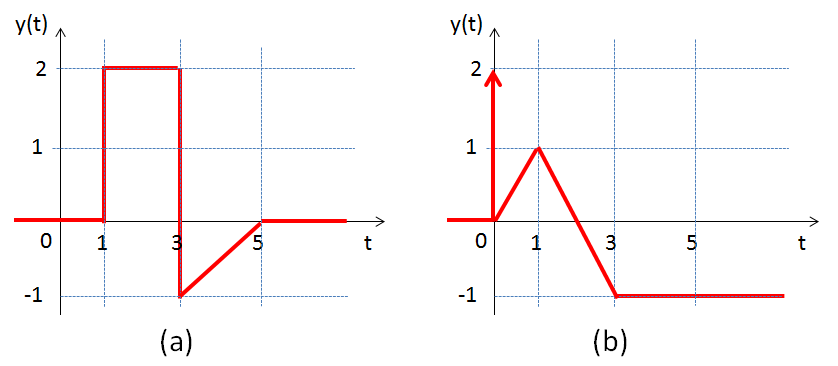
\includegraphics[scale=0.5]{images/Exo_2_2.jpg} 
	\end{figure} 

	
	2. Réécrivez sous la forme d'une fonction à valeurs réelles les fonctions suivantes et esquissez leur forme temporelle (pour t >0) :
	
	a. $x(t) = (1+j)e^{j\cdot 10t}$ 
	
	b. $y(t) = e^{(-2+j)t}\cdot u(t-2)$ 
	
	c. $z(t) = e^{(-1+2j)t}+e^{(-1-2j)t}$
	
	\vspace{1\baselineskip} 
	
	
	\subsubsection{Exercice 3 - Réponse indicielle d'un circuit RC}
	
	On reprend le circuit RC dont on a étudié la réponse dans la partie VI.3. On considère deux cas : celui où le condensateur est déchargé initialement, puis celui où il est chargé. 
	
	a. Calculez la réponse naturelle du circuit lorsque le condensateur est initialement chargé.
	
	b. En déduire la réponse impulsionnelle du circuit.
	
	c. Calculez la réponse lorsque le circuit est soumis à un échelon de Heaviside d'amplitude E, dans les deux cas (charge initiale absente ou présente).
	
	d. En déduire la réponse indicielle du circuit.
	
	\vspace{1\baselineskip}	
	

	
	\subsubsection{Exercice 4}
	
	On considère les deux circuits électriques ci-dessous. Pour le circuit (a), la tension initiale (t=0) aux bornes du condensateur C est notée $U_{C0}$. Pour le circuit (b), un courant noté $I_L0$ traverse la bobine L. La sortie de ces deux circuits est la tension $U_{S}$.
	
	\begin{figure}[h!]
		\centering
		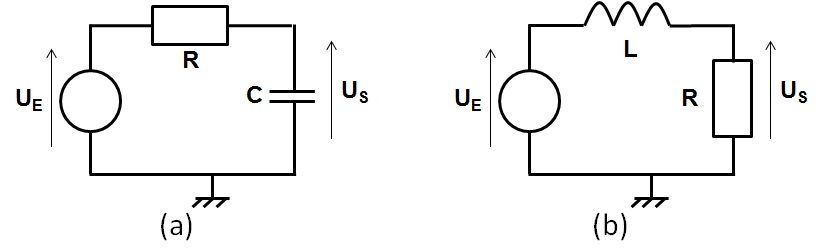
\includegraphics[scale=0.5]{images/Exo_2_4.jpg} 
	\end{figure} 
	
	a. Déterminez les fréquences et les réponses naturelles de ces deux circuits. Quel est l'ordre de ces deux systèmes ? 
	
	b. On excite ces deux systèmes à l'aide d'un échelon de Heaviside d'amplitude notée E. Déterminez la réponse indicielle de ces deux circuits. 
	
	c. Déterminez les fonctions de transfert de ces deux circuits.
	
	\vspace{1\baselineskip}
	
	\subsubsection{Exercice 5 - Fonction de transfert d'un circuit résonant}
	
	On reprendre le circuit RLC présenté dans la partie IV.4. Celui-ci est excité par un générateur de courant I, comme le montre la figure ci-dessous. On s'intéresse à la tension U aux bornes de ce circuit RLC. 
	
	\begin{figure}[h!]
		\centering
		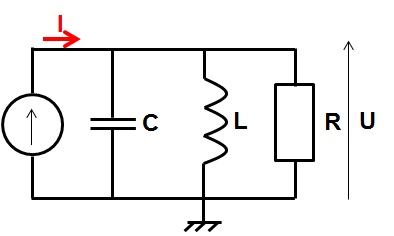
\includegraphics[scale=0.5]{images/Exo_2_5.jpg} 
	\end{figure} 
	
	a. Déterminez la fonction de transfert de ce circuit. 
	
	b. Précisez l'unité de la fonction de transfert. 
	
	c. Dans le cas où l'on considère une excitation cosinusoïdale du circuit, y a t-il une fréquence particulière où la réponse présente un maximum ? Si oui, laquelle ? Donnez l'expression de la réponse temporelle du circuit en régime permanent.
	
	\vspace{1\baselineskip}
	
	\subsubsection{Exercice 6}
	
	On considère le système dont le fonctionnement est décrit par le schéma-bloc ci-dessous. Celui-ci transforme un signal d'entrée e(t) et délivre en sortie un signal s(t). 
	
	\begin{figure}[h!]
		\centering
		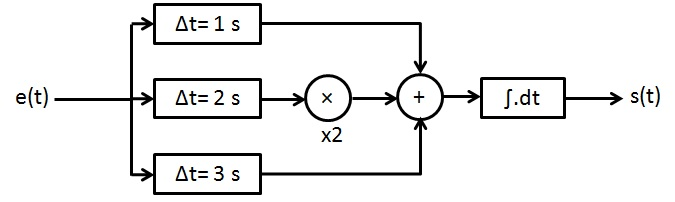
\includegraphics[scale=0.5]{images/Exo_2_6.jpg} 
	\end{figure}
	
	a. Le système est-il linéaire, à temps invariant, causal ?
	
	b. Déterminez l'expression de la réponse impulsionnelle h(t) du système. Esquissez l'allure temporelle de la réponse impulsionnelle. 
	
	c. Déterminez l'expression de la fonction de transfert H(p) du système. Précisez les pôles et les zéros de la fonction de transfert. Que concluez-vous sur sa stabilité ?
	
	\vspace{1\baselineskip}
	
	Question bêbête : est-ce que les termes suivants sont justes : un système linéaire à temps variant, un signal non linéaire, un signal non causal.


	\newpage
	
	
\chapter{Transformée de Laplace}	
	
	
	Dans le chapitre précédent, nous avons identifié deux manières de calculer la réponse transitoire d'un système :
	\begin{itemize}
		\item soit en considérant la réponse impulsionnelle et en calculant le produit de convolution dans le domaine temporel
		\item soit en considérant la fonction de transfert et en réalisant une simple multiplication dans le domaine fréquentiel, nécessitant une excitation exponentielle complexe.
	\end{itemize}

	Bien que cette deuxième méthode soit plus simple, elle suppose une excitation d'un type donné. La question posé et qui est illustré ci-dessous est : peut-on passer directement d'une fonction temporelle à sa forme dans le domaine fréquentiel complexe, même si celle-ci n'est pas une exponentielle complexe ? Nous allons voir que cela est possible, via une transformation mathématique appelée transformée de Laplace. En plus de nous offrir un moyen pratique pour déterminer les réponses des systèmes quel que soit le type d'excitation, nous verrons  qu'elle permet de résoudre d'une manière pratique les équations différentielles ordinaires, quel que soit leur ordre (on pourra remarquer qu'il s'agit en fait du même problème). 
	
	\begin{figure}[h!]
		\centering
		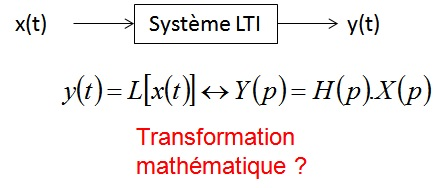
\includegraphics[scale=0.5]{images/Position_Pb_Laplace.jpg}
		\caption{Construction de la réponse impulsionnelle}	
		\label{Fig:Position_Pb_Laplace} 
	\end{figure}
	
	 La transformée de Laplace permet de passer du domaine temporel à son domaine dual, le domaine fréquentiel. Dans les chapitres suivants, nous présenterons un autre type de transformation dérivée de la transformée de Laplace : la transformée de Fourier, qui sera très utile pour l'analyse des signaux, ainsi que pour l'étude des systèmes en régime permanent.
	
	\vspace{0.5\baselineskip}
	\underline{Remarque :}
	Dans ce chapitre, on ne considère que des fonctions causales. L'instant d'apparition des signaux se fera en t = 0. Pour représenter cette condition, l'ensemble des signaux en entrée et en sortie que nous allons considérer seront multiplier par l'échelon de Heaviside u(t).
	\vspace{1\baselineskip}
	
	\section{Dérivation d'une transformation d'une fonction temporelle au domaine fréquentiel}
	Dans le domaine temporel, l'entrée et la sortie du système sont reliés par la réponse impulsionnelle h(t) et le produit de convolution. Cela est vrai quel que soit le type d'excitation appliquée en entrée du système. Le passage dans le domaine fréquentiel suppose une excitation exponentielle complexe. Considérons ce cas dans le domaine temporel : la réponse sera donc égale au produit de convolution entre la réponse impulsionnelle et l'excitation exponentielle complexe. Nous considérons dans un premier temps un signal défini sur tout le domaine temporel. Elle peut être modifiée selon la forme donnée par l'équation \ref{Demo_Laplace}.
	
	\begin{equation}\label{}
	y(t) = h*x(t) = h * exp(pt) = \int_{-\infty}^{+\infty} h(\tau) \cdot exp(p(t-\tau))
 \deriv \tau 	
 	\end{equation}
	\begin{equation}\label{Demo_Laplace}
	y(t) = exp(pt) \int_{-\infty}^{+\infty} h(\tau) \cdot exp(-p\tau)
	\deriv \tau 	
	\end{equation}
	
	On remarque que la réponse du système est le produit entre l'excitation et un terme intégrale dépendant de la réponse impulsionnelle. On retrouve donc une forme très similaire à celle vue à l'équation \ref{Def_fonction_tranfert}, reliant réponse et excitation exponentielle complexe, via la fonction de transfert. Ce terme intégrale n'est donc rien d'autre que la réponse du système LTI dans le domaine fréquentiel complexe, c'est-à-dire sa fonction de transfert.
	\begin{figure}[h!]
		\centering
		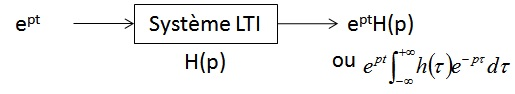
\includegraphics[scale=0.7]{images/LTI_Laplace.jpg}
		\caption{Lien via la transformée de Laplace entre l'excitation exponentielle complexe et la réponse d'un système LTI}	
		\label{Fig:LTI_Laplace} 
	\end{figure}
	
	Nous venons de mettre en évidence une transformation mathématique permettant de passer de la représentation temporelle d'une fonction à sa représentation fréquentielle complexe. Cette transformée s'appelle la transformée de Laplace. Elle est donnée par \ref{Fonction_Transfert_Laplace_non_causale} dans le cas général.
	\begin{equation}\label{Fonction_Transfert_Laplace_non_causale}
	H(p) = \int_{-\infty}^{+\infty} h(t) \cdot exp(-pt)	\deriv t~,~~p \in \mathbb{C}	
	\end{equation}	
	
	La démonstration précédente reste valable dans le cas d'un signal causal, défini pour t > 0. Dans ce cas, on peut écrire :
	\begin{equation}\label{Fonction_Transfert_Laplace_causale}
	H(p) = \int_{0}^{+\infty} h(t) \cdot exp(-pt)	\deriv t~,~~p \in \mathbb{C}	
	\end{equation}
	
	\section{Transformée de Laplace}
	\subsection{Définition}
	La transformée de Laplace est une transformation mathématique, transformant une fonction temporelle en une fonction définie dans le domaine des fréquences complexes p. Nous noterons $\mathcal{L}$ cette transformation. On distingue deux types de transformée de Laplace : bilatérale (\ref{Transfo_Laplace_non_causal}) et unilatérale (\ref{Transfo_Laplace_causale}). Cette dernière s'impose naturellement dès que l'on considère des systèmes causaux (h(t) = 0 pour t <0). Dans la suite, comme nous ne traiterons que de systèmes causaux, nous ne considérerons que la transformée de Laplace unilatérale.
	\begin{equation}\label{Transfo_Laplace_non_causale}
	F(p) = \mathcal{L}[f(t)] = \int_{-\infty}^{+\infty} f(t) \cdot exp(-pt)	\deriv t~,~~p=\sigma + j \omega	
	\end{equation}
	\begin{equation}\label{Transfo_Laplace_causale}
	F(p) = \mathcal{L}[f(t)] = \int_{0^{+}}^{+\infty} f(t) \cdot exp(-pt)	\deriv t~,~~p=\sigma + j \omega	
	\end{equation}

	
	\subsection{Conditions d'existence de la transformée de Laplace et stabilité des systèmes}
	Il est important de noter que la transformée de Laplace n'existe que si l'intégrale converge. Ceci n'est pas le cas pour toutes les valeurs de p.
	L'objectif de ce cours n'est pas de faire ce calcul intégrale, mais plutôt de l'utiliser comme outil pour l'étude des systèmes linéaires. Nous utiliserons la plupart du temps des tables contenant les transformées pour les fonctions les plus courantes. Néanmoins, nous allons mettre en œuvre ce calcul à travers un exemple et indiquer les conditions d'existence de la transformée de Laplace. Nous allons mettre en évidence ce que cela signifie du point de vue de la stabilité des systèmes LTI. Par souci de simplification, on dira qu'un système est stable si il converge vers une valeur finie.
	Exemple : nous considérons un système LTI dont la réponse impulsionnelle est définie par la fonction : $h(t) = exp(\alpha t)u(t) $ où $\alpha$ est un réel quelconque.
	Calculons sa transformée de Laplace à l'aide de l'équation \ref{Transfo_Laplace_non_causale} :
	\begin{equation*}
	H(p) = \mathcal{L}[exp(\alpha t)u(t)] = \int_{-\infty}^{+\infty}exp(\alpha t)u(t) \cdot exp(-pt) \deriv t
	\end{equation*}
	\begin{equation*}
	H(p) = \int_{0}^{+\infty}exp(-(p-\alpha) t) \deriv t
	\end{equation*}
	\begin{equation*}
	H(p) = \lim_{T \to +\infty} \frac{1-exp(-(p-\alpha)T)}{p-\alpha} = \lim_{T \to +\infty} \frac{1-exp(-(\sigma-\alpha)T)exp(-j\omega T)}{p-\alpha}
	\end{equation*}
	La transformée de Laplace existera si cette intégrale converge, donc cela dépend de la partie réelle $\sigma$ de la fréquence complexe :
	\begin{equation}\label{}
	F(p) = \left \{
	\begin{array}{l l}
	\frac{1}{p-\alpha}  & si~\sigma>\alpha \\
	\infty   & sinon \\
	\end{array}
	\right .	 	
	\end{equation}
	
	Si on représente l'excitation en fréquence dans le plan p, il existe un
	domaine d'existence de la transformée de Laplace appelé domaine de
	convergence. Il s'agit d'un plan où Re(p) = $\sigma $ \textgreater{} $\alpha $. Nous le
	représentons dans deux cas différents :  $\alpha $ \textless{} 0 et  $\alpha $
	\textgreater{} 0. Nous allons analyser la signification concrète de ce
	domaine de convergence.
	\begin{figure}[h!]
		\centering
		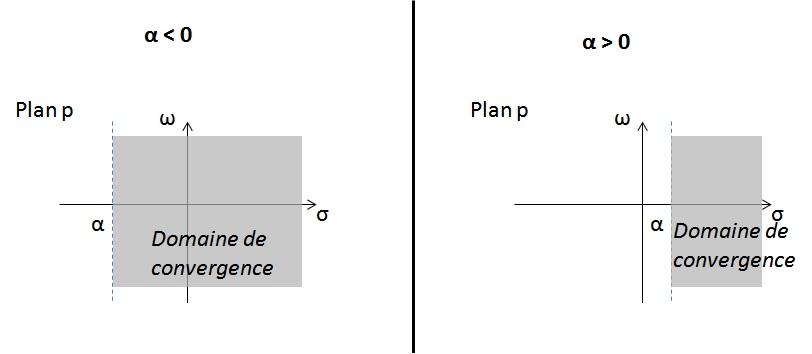
\includegraphics[scale=0.8]{images/Domaine_convergence_exp_at.jpg}
		\caption{Domaine de convergence de la fonction $exp(\alpha t)$}	
		\label{Fig:Domaine_convergence_exp_at} 
	\end{figure}
	Le domaine de convergence indique, dans le cas d'une excitation
	exponentielle complexe, l'ensemble des fréquences complexes pour lequel
	le système convergera (que l'entrée converge ou pas !). Pour s'en
	convaincre, considérons une excitation exponentielle, de fréquence
	complexe $p_{0} =  \beta +j \omega $. Reprenons la forme initiale dérivée de la réponse	impulsionnelle.
	\begin{equation*}
	y(t) = exp(p_{0}t)\int_{-\infty}^{+\infty}h(\tau)exp(-p_{0}\tau) \deriv \tau 
	\end{equation*}
	\begin{equation*}
	y(t) = exp((\beta+j\omega)t)\int_{-\infty}^{+\infty}exp(\alpha \tau)exp(-(\beta+j\omega)\tau) \deriv \tau 
	\end{equation*}
	\begin{equation*}
	y(t) = exp((\beta+j\omega)t)\int_{-\infty}^{+\infty}exp(-(\beta-\alpha+j\omega)\tau) \deriv \tau 
	\end{equation*}
	\begin{equation}
	y(t) = \lim_{T \to +\infty} \frac{exp((\beta+j\omega)t)(exp(-(\beta-\alpha+j\omega)T)-1)}{\beta-\alpha+j\omega} 
	\end{equation}
	Cette fonction converge bien si la partie réelle $\beta $ de la fréquence de
	l'excitation est supérieure à  $\alpha $, autrement dit si la fréquence complexe
	d'excitation appartient au domaine de convergence, mais aussi si $\beta $
	\textless{} 0. Dans le cas contraire le signal d'entrée va diverger pour
	t \textgreater{} 0. Cette double condition sur $\beta $ n'est possible que si $\alpha $
	\textless{} 0, qui est donc une condition nécessaire pour que le système
	soit stable.
	
	\underline{Remarque : cas d'une excitation harmonique :}
	Cette situation correspond au cas où $\beta $ = 0. Le système sera stable
	uniquement si, dans le plan p, l'axe des imaginaires appartient au
	domaine de convergence. Dans le chapitre consacré à la transformée de
	Fourier, nous verrons qu'elle est équivalente à une transformée de
	Laplace, mais pour une fréquence purement complexe $\beta $ = 0. Si l'axe des
	imaginaires appartient au domaine de convergence, alors la transformée
	de Fourier de la fonction pourra exister.
	
	\subsection{Pôles et zéros d'une fonction de transfert}
	
	Reprenons l'exemple précédent. Comme nous l'avions introduit dans le
	chapitre précédent, $\alpha $ correspond à un pôle de la réponse du système. Sa
	stabilité est liée à sa partie réelle.~
	
	Toutes les trasnformées de Laplace que l'on considère peuvent se mettre sous la forme d'une
	fonction rationnelle, où le numérateur N(p) et dénominateur D(p) sont
	des polynômes. Eux-mêmes peuvent être exprimés en fonction de leurs
	racines appelés zéros et pôles respectivement. Ceux-ci correspondent à
	des fréquences complexes particulières qui :
	\begin{itemize}
		\item annulent la fonction de transfert dans le cas des zéros p\textsubscript{zi}
	
		\item font tendre la fonction de transfert vers l'infini dans le cas des pôles p\textsubscript{pj}
	\end{itemize}
	
	\begin{equation}\label{key}
	F(p) = \frac{N(p)}{D(p)} = \frac{b_{m}p^{m}+...+b_{1}p+b_{0}}{a_{n}p^{n}+...+a_{1}p+a_{0}} ~\Rightarrow ~ F(p) = G \frac{\prod_{i=0}^{m}(p-p_{zi})}{\prod_{i=0}^{n}(p-p_{pj})}
	\end{equation}
	où G est le gain de la fonction de transfert.
	Comme nous l'avions déjà vu dans le chapitre A, la position des pôles nous donne une indication sur l'allure temporelle de la fonction de transfert (réponse naturelle).
	Quel que soit le système linéaire considéré, la position de ces pôles va déterminer la stabilité du système. Vous approfondirez ces concepts dans le cours d'automatique.
	
	\section{Propriétés de la transformée de Laplace}
	Dans cette partie, nous allons passer en revue plusieurs des propriétés importantes de la transformée de Laplace, qui facilitent les calculs de la transformée de Laplace et les applications associées. Nous ne démontrerons pas l'ensemble de ces propriétés.
	\subsection{Linéarité}
	La transformée de Laplace est linéaire. La transformée de Laplace d'une somme pondérée de fonction est la somme des transformées de Laplace individuelle de ces fonctions, pondérées de la même manière. Elle vérifie donc la relation suivante.
	\begin{equation}\label{key}
	a \cdot f(t)+b \cdot g(t) \longleftrightarrow a \cdot F(p)+b \cdot G(p)
	\end{equation}
	
	\subsection{Théorème du retard}
	
	Supposons que l'on connaisse la transformée de Laplace F(p) de la
	fonction causale f(t), qui est nulle pour t \textless{} 0. Si on a
	retardé de t\textsubscript{0} cette fonction, elle devient
	f(t-t\textsubscript{0}) celle-ci est nulle pour tout t \textless{}
	t\textsubscript{0}. Calculons sa transformée de Laplace à partir de xxx
	et appliquons le changement de variable w = t-t\textsubscript{0}. On
	montre que la transformée de Laplace de la fonction retardée est la
	transformée de Laplace non retardée multipliée par
	e-\textsuperscript{pt0}.
	
	\begin{equation*}
	F_{t0}(p) = \mathcal{L}[f(t-t_{0})]=\int_{t_{0}}^{+\infty}f(t-t_{0})exp(-pt) \deriv t   
	\end{equation*}
	\begin{equation*}
	F_{t0}(p) = \int_{0}^{+\infty}f(w)exp(-p(w+t_{0})) \deriv w = \int_{0}^{+\infty}f(w)exp(-pw)exp(-pt_{0}) \deriv w  
	\end{equation*}
	\begin{equation}\label{}
	F_{t0}(p) = F(p)\cdot exp(pt_{0})
	\end{equation}
	
	\subsection{Théorème du changement d'échelle}
	
	Supposons que l'on connaisse la transformée de Laplace F(p) de la
	fonction causale f(t). Dilatons l'échelle de temps de cette fonction par
	un facteur réel k. La fonction devient f(kt). Calculons la transformée
	de Laplace de cette version dilatée de f(t), en appliquant le changement
	de variable $w = kt$.
	\begin{equation*}
	F_{k}(p) = \mathcal{L}[f(kt)]=\int_{t_{0}}^{+\infty}f(kt)exp(-pt) \deriv t  =\int_{t_{0}}^{+\infty}\frac{1}{k}f(w)exp(-\frac{p}{k}w) \deriv w 
	\end{equation*}
	\begin{equation}\label{}
	F_{k}(p) = \frac{1}{k}\cdot F(\frac{p}{k})
	\end{equation}
	
	\subsection{Dérivation dans le domaine temporel}
	Considérons le cas d'une fonction f(t) continue non nulle pour t > 0. La transformée de Laplace de la dérivée de cette fonction est donnée par :
	Attention : 0moins ou 0plus ?
	\begin{equation}\label{key}
	\mathcal{L}[\frac{df}{dt}] = p\cdot F(p)-f(0^{+}) ~~~avec~f(0^{+})=\lim_{t\rightarrow0^{+}}f(t)
	\end{equation}

	On remarque que l'opérateur dérivée correspond à une multiplication de
	la transformée de Laplace par p. Cependant, il est nécessaire de tenir
	compte de la condition initiale f(0\textsuperscript{+}).
	
	Il est possible de généraliser cette relation au cas où l'on dérive N
	fois. L'expression devient :
	\begin{equation}\label{key}
	\mathcal{L}[\frac{d^{n}f}{dt^{n}}] = p^{n}\cdot F(p)-p^{n-1}\cdot f(0^{+})-p^{n-2}\cdot \frac{df}{dt}(0^{+})-...-p\frac{d^{n-2}f}{dt^{n-2}}(0^{+})-\frac{d^{n-1}f}{dt^{n-1}}(0^{+})
	\end{equation}
	Le calcul nécessite de connaître les conditions initiales non seulement sur la valeur de la fonction mais sur ses (n-1) premières dérivées.
	
	\subsection{Dérivation dans le domaine des fréquences complexes p}
	
	\subsection{Intégration temporelle}
	Si une fois et si N fois
	
	\subsection{Théorème de la valeur initiale}
	
	\subsection{Théorème de la valeur finale}
	
	\subsection{Multiplication et produit de convolution}
	
	\subsection{Fonctions périodiques causales}
	
	\subsection{Fonctions causales avec N répétitions}
	En lien avec la propriété précédente
	
	\subsection{Tableau récapitulatif des propriétés}
	Tableau 5.1 du livre Y. Mori.
	Uniquement les plus importantes.
	
	
	\section{Transformée de Laplace des fonctions courantes}
	Le tableau ci-dessous donne la transformée de Laplace des fonctions causales les plus courantes, et pour lesquelles des formes mathématiques simples existent. Pour la plupart, aucune démonstration n'est donnée, mais les transformées peuvent être retrouvées. Nous nous limiterons à deux exemples de mise en forme de la transformée de Laplace pour deux formes temporelles courantes, sachant que nous avons déjà vu celle d'une fonction exponentielle.
	
	\underline{Exemple 1 : échelon unitaire f(t) = u(t)}
	\begin{equation*}
	F(p)=\mathcal{L}[u(t)] = \int_{-\infty}^{+\infty}u(t)exp(-pt) \deriv t =\int_{0}^{+\infty}exp(-pt) \deriv t = [-\frac{exp(pt)}{p}]_{0}^{+\infty}=\frac{1}{p}
	\end{equation*}
	
	\underline{Exemple 2 : fonction cosinusoïdale}
	\begin{equation*}
	f(t)=cos(\omega t)u(t)
	\end{equation*}
	\begin{equation*}
	F(p)=\mathcal{L}[f(t)]=\int_{-\infty}^{+\infty}cos(\omega t)u(t) \deriv t=\int_{0}^{+\infty}\frac{exp(j\omega t)+exp(-j\omega t)}{2} \deriv t
	\end{equation*}
	\begin{equation*}
	F(p)=\frac{1}{2}\int_{0}^{+\infty}(exp((j\omega-p) t)+exp(-(j\omega+p) t)) \deriv t=\frac{1}{2}([\frac{exp((j\omega-p) t)}{j\omega-p}]_{0}^{+\infty}-[\frac{exp((j\omega-p) t)}{j\omega-p}]_{0}^{+\infty})
	\end{equation*}
	\begin{equation}\label{}
	F(p)=\frac{1}{2}(-\frac{1}{j\omega-p}+\frac{1}{j\omega+p})=\frac{p}{p^{2}+\omega^{2}}
	\end{equation}
	
	\underline{Tableau récapitulatif des transformées de Laplace :}
	
	\begin{table}[h]
		\centering
		\caption{\label{Tab:Transfo_Laplace_usuelle} Tableau récapitulatif des transformées de Laplace usuelles}
		\begin{tabular}{|l|c|}
			\hline
			\textbf{Fonctions temporelles f(t)} & \textbf{Transformée de Laplace F(p)} \\
			\hline
			Echelon unitaire u(t) & $\frac{1}{p}$ \\	
			\hline
			Fonction rampe $f(t)=t\cdot u(t)$ & $\frac{1}{p^{2}}$ \\	
			\hline
			Fonction rampe polynomiale $f(t)=\frac{t^{n-1}}{(n-1)!} u(t)$ & $\frac{1}{p^{n}}$ \\	
			\hline
			Fonction exponentielle $f(t)=e^{-\alpha t} u(t)$ & $\frac{1}{p+\alpha}$ \\	
			\hline
			$f(t)=te^{-\alpha t} u(t)$ & $\frac{1}{(p+\alpha)^{2}}$ \\
			\hline
			$f(t)=\frac{t^{n-1}}{(n-1)!}e^{-\alpha t} u(t)$ & $\frac{1}{(p+\alpha)^{n}}$ \\
			\hline
			Fonction cosinus $f(t)=cos(\omega t)u(t)$ & $\frac{p}{p^{2}+\omega^{2}}$ \\
			\hline
			Fonction sinus $f(t)=sin(\omega t)u(t)$ & $\frac{\omega}{p^{2}+\omega^{2}}$ \\
			\hline
			Fonction cosinus amorti $f(t)=e^{-\alpha t}cos(\omega t)u(t)$ &  $\frac{p+\alpha}{(p+\alpha)^{2}+\omega^{2}}$ \\
			\hline
			Fonction rampe limitée $f(t)= \left\{\begin{array}{l}
			A\frac{t}{\tau}u(t)~,~si~t \leq \tau \\
			A\cdot u(t) \\
			\end{array} 
			\right . $ & $A\frac{1-e^{-p\tau}}{p^{2}\tau}$ \\
			\hline
		\end{tabular}	
	\end{table}


	A partir de cette table, il est possible de dériver les transformées de Laplace pour d'autres fonctions temporelles. En effet, il suffit d'identifier des formes dont la transformée de Laplace est connue et utiliser les différentes propriétés de la transformée pour en déduire l'expression de la transformée de Laplace.
	
	Exemple : cas composé de plusieurs formes connues~ par exemple trois
	marches d'escalier, avec transition en t = 0, 1, 2 (exo 3-a p 108 Y.
	Mori) : solution : $f(t) = F(p) = u(t) + u(t-1) + u(t-2) - 3u(t-3) \Rightarrow F(p)
	=1/p+e\textsuperscript{-p}/p+e\textsuperscript{-2p}/p-3e\textsuperscript{-3p}/p$
	
	
	\section{Transformée de Laplace inverse}
	\subsection{Méthode}
	Du point de vue pratique, le but de la transformée de Laplace est de fournir un outil simple pour le calcul des réponses temporelles des systèmes linéaires. Elle permet de calculer la représentation fréquentielle d'une fonction à partir de sa représentation dans le domaine temporel. Dans le domaine fréquentiel, le calcul de la réponse du système est facilité en passant par la fonction de transfert. Cependant, si nous ne disposons pas d'une transformation mathématique permettant de réaliser le passage inverse, cette approche perd de son intérêt.  Fort heureusement, cet outil existe. Il s'agit de la transformée de Laplace inverse, que nous allons rapidement présenter. 
	La transformée de Laplace inverse est donnée par la formule de Bromwich-Mellin , où $\sigma$ est choisi pour que l'intégrale converge.
	
	\begin{equation}\label{TL_inverse}
	f(t) = \mathcal{L}^{-1}[F(p)]=\frac{1}{2\pi j}\int_{\sigma - j\infty}^{\sigma + j\infty}F(p)exp(pt) \deriv p
	\end{equation}
	
	Dans la pratique, cette formule est difficile à mettre en œuvre car elle nécessite de calculer une intégrale dans le plan complexe. Ceci dépasse le cadre de ce cours et nous n'effectuerons pas de calcul de cette transformée. Dans ce cours, nous privilégierons la méthode utilisée en pratique, basée sur les tables reliant des fonctions courantes et leur transformée de Laplace, comme le tableau xx. Il s'agit de rechercher des paires de transformées. A partir de la fonction F(p), on identifie des fonctions connues et on déduit la fonction temporelle correspondante. Dans le cas de fonctions compliquées, le calcul de la forme temporelle passe par des approches basées sur le calcul numérique, non détaillées ici.
	
	\subsection{Décomposition pôles-résidus}
	Comme nous l'avons dans la partie II.3, la plupart des transformées de Laplace peuvent être mis sous la forme d'une fonction rationnelle, rapport de deux polynômes faisant apparaitre leurs racines (pôles et zéros). Cependant, il n'existe sans doute pas une paire de transformées simple pour toutes les fonctions rationnelles. Pour appliquer la méthode précédente, il est nécessaire de décomposer cette fonction rationnelle en éléments plus simple, dont on connait la paire de transformée.
	Il est possible de montrer que toute fonction rationnelle de deux polynômes peut s'écrire sous la forme d'une somme d'éléments simples, appelées fractions partielles ne dépendant que des pôles et de constantes appelées résidus. Cette décomposition s'appelle décomposition pôles-résidus. 
	
	Forme après décomposition pôles-résidus
	
	On voit immédiatement l'intérêt de cette approche car on remarque qu'on identifie immédiatement la paire de transformée simple. En effet, la transformée de Laplace inverse de la fraction partielle est une fonction exponentielle, dépendante du pôle (remarque : on retrouve l'expression temporelle de la réponse naturelle vue dans le chapitre A).
	
	Méthode : cas où n >= m et cas où n < m
	Méthode du cache : vue en première année.
	
	\subsection{Exemple}
	
	\section{Applications} 
	Nous allons présenter deux applications où l'utilisation de la transformée de Laplace et de son inverse trouve tout leur intérêt : dans la résolution d'équations différentielles et dans le calcul de la réponse transitoire de systèmes linéaires.
	\section{Résolution d'équations différentielles ordinaires}
	Les équations différentielles ordinaires s'écrivent de la manière générale suivante. Elles résultent de l'effet d'opérateurs proportionnels, intégrateurs et différentiateurs. Dans le domaine des fréquences complexes, ces deux derniers effets se résument à une multiplication et une division par la fréquence p. On constate qu'en passant dans le domaine fréquentiel, l'équation différentielle se transforme en une simple simple équation algébrique. On retrouve bien que les fonctions Y(p) et X(p) sont reliées par un terme H(p) qui est la fonction de transfert et qui ne dépend que des coefficients ai et aj. Une fois l'expression de la fonction de transfert établie, on peut calculer la solution Y(p) de l'équation différentielle pour toute excitation X(p) (à condition que l'on puisse calculer la transformée de Laplace de x(t)). On pourra déterminer ensuite la solution y(t) dans le domaine temporel à l'aide de la transformée de Laplace inverse.
	\begin{figure}[h!]
		\centering
		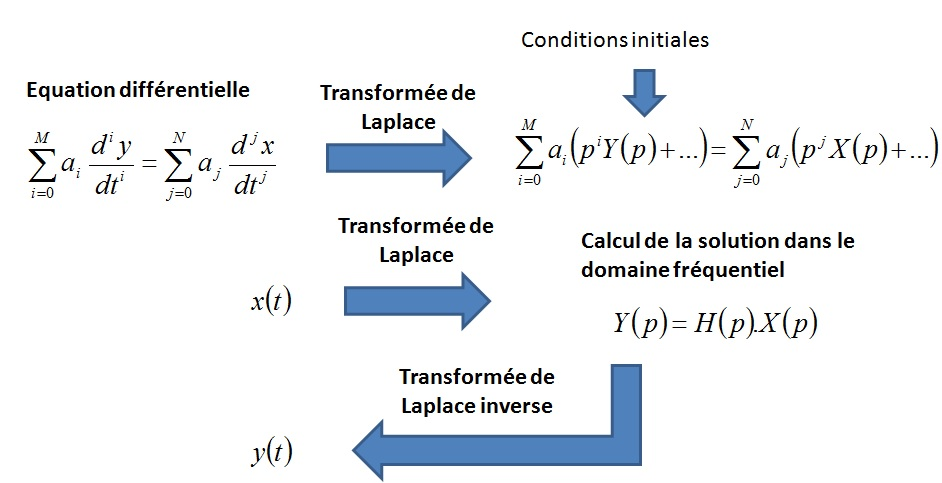
\includegraphics[scale=0.6]{images/Methodo_reso_equa_diff_Laplace.jpg}
		\caption{Méthodologie de résolution d'une équation différentielle ordinaire basée sur la transformée de Laplace}	
		\label{Fig:Methodo_reso_equa_diff_Laplace} 
	\end{figure}
	Exemple : soit l'équation différentielle … avec comme conditions initiales …
	
	\subsection{Calcul de la réponse transitoire d'un système linéaire}
	Comme le comportement transitoire d'un système est dicté par une équation différentielle, déterminer la réponse temporelle à une excitation donnée revient à résoudre cette équation différentielle. Le problème est donc équivalent au précédent. Supposons que nous disposions de la fonction de transfert H(p) du système et que l'on recherche la réponse y(t) à une excitation x(t) dont l'expression est donnée. La première étape consiste à déterminer la transformée de Laplace X(p) de l'excitation. La réponse du système dans le domaine fréquentiel Y(p) est directement le produit de la fonction de transfert et de l'excitation X(p). Ensuite, la transformée de Laplace inverse de Y(p) permet de retrouver l'expression de la réponse temporelle y(t).
	Il est bien entendu indispensable de prendre en compte les conditions initiales du système, qui vont intervenir dans la réponse naturelle du système. Si l'expression de la fonction de transfert ne les intègre pas, il est indispensable de repartir de l'équation différentielle décrivant le système et établir la fonction de transfert en intégrant l'effet des conditions initiales.
	Exemple : on considère un système dont la fonction de transfert est donnée par … On souhaite calculer sa réponse à l'excitation x(t) = … Les conditions initiales sont …
	
	
	On reprend l'exemple du circuit RC vu dans le chapitre précédent. On considère qu'il est excité par un échelon unitaire en t = 0, et que le condensateur est initialement chargé. On souhaite déterminer la réponse du circuit, correspondant à la tension aux bornes de la résistance.
	
	\section{Ce qu'il faut retenir}
	
	\section{Exercices}
	
	
	
	\subsubsection{Exercice 6}
	
	On reprend l'exercice 6 du chapitre 2.

	
	\begin{figure}[h!]
		\centering
		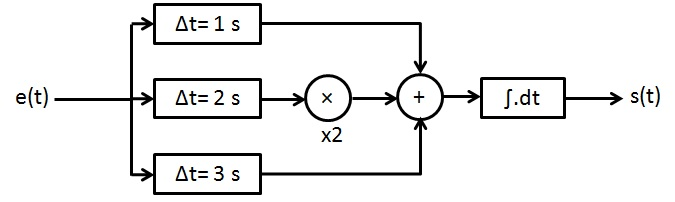
\includegraphics[scale=0.5]{images/Exo_2_6.jpg} 
	\end{figure}
	
	a. Ecrivez la fonction de transfert du système dans le domaine de Laplace.
	
	b. Calculez la réponse indicielle du système. On supposera que les conditions initiales de tous les nœuds internes du système sont nulles. 
	
	
	\vspace{1\baselineskip}
	
	\subsubsection{Exercice 6}
	
	On considère un circuit électrique, dont le courant i(t) est donné par l'équation ci-dessous.
	\begin{equation*}
	e(t)=\frac{d^{2}i}{dt^{2}}+7\frac{di}{dt}+10i(t)
	\end{equation*}
	On considère l'excitation suivante $e(t)=6e^{-3t}u(t)$. Les conditions initiales du circuit sont : $i(0) = 3~A$ et $\frac{di}{dt}(0)=3~A/s$.
	
	
	a. Etablir l'expression du courant dans le domaine de Laplace.
	
	b. En déduire l'expression temporelle du courant i(t).
	
	c. Vérifiez, en utilisant les expressions du courant dans le domaine de Laplace, puis dans le domaine temporel, que la condition initiale du courant est respectée. Déterminez ensuite les conditions finales. 
	
	\vspace{1\baselineskip}
	
	
	
	
	
	\newpage
	
	
	
	
\chapter{Filtrage}

	Ici, uniquement dans le domaine fréquentiel. L'analyse dans le domaine
	temporel sera vue dans le chapitre xxx, et utilisera la réponse
	impulsionnelle.
	
	analyse du comportement fréquentiel d'un système linéaire~ on considère
	le cas d'une excitation purement harmonique. Définition des différents
	types de filtre, gabarit fréquentiel et caractéristiques associées
	(bande passante, ordre, fréquence de coupure).
	
	On considère le régime harmonique établi~ p = j$\omega$. Ici, l'analyse
	harmonique va jouer un rôle majeur dans l'analyse fréquentielle des
	filtres.
	
	A partir de la fonction de transfert dans le domaine de Laplace : H(p)~
	H(j$\omega$) ou H(f).
	
	Dans la suite, par souci de simplification, nous parlerons de fréquence
	f au lieu de pulsation $ \omega $. La fonction de transfert ne sera pas notée
	H(j$ \omega $) mais H(f).
	
	\section{Définition d'un filtre}
	Un filtre est un système présentant une certaine sélectivité dans le domaine des fréquences, et qui est donc utilisé pour limiter le spectre d’un signal à une certaine bande de fréquences.
	Un filtre atténue certaines des composantes fréquentielles du signal d’entrée et en laisse passer d’autres, d’où son appellation de filtre ! C’est bien cette opération sélective d’atténuation ou d’amplification des fréquences que modélise la multiplication de l'excitation par la fonction de transfert.
	\begin{equation}\label{}
	Y(f) = H(f) \cdot X(f)
	\end{equation}

	La fonction de transfert peut s'écrire : $ H(f) = |H(f)|exp(j~arg(H(f)))$, qui se décompose sous la forme d'un module et d'un argument. Le module correspond au gain du filtre, c'est-à-dire le rapport entre le module de la réponse du filtre sur celui de son excitation. Si les signaux d'entrée et de sortie représentent le même type de grandeur (par exemple, une tension dans le cas de signaux électriques), le gain est sans unité. L'argument correspond au déphasage apporté par le filtre.
	
	retard : le déphasage traduit un retard $ \tau $, dépendant de la fréquence,
	qui se calcule de la manière suivante : Vérifier la formule car une
	phase \textless{} 0 va donner $\tau$ \textless{} 0. Or, si tau est un
	retard, alors il devient une avance dans cette situation.
	\begin{equation}\label{}
	\tau = \frac{Arg(H(f))}{2\pi f}
	\end{equation}
	Un déphasage constant quelque soit la fréquence n'est pas réalisable en pratique…
	
	On remarque une propriété intéressante : soit un signal est constitué de la superposition de plusieurs signaux sinusoïdaux, qui traverse un filtre présentant un déphasage variable en fonction de la fréquence. Même si le gain est le même à ces différentes fréquence, si le retard introduit par le filtre n'est pas le même, alors le signal présentera une distorsion.
	Cependant, si le déphasage varie linéairement avec la fréquence, on remarque que le retard sera constant. Dans la situation précédente, la distorsion disparaîtra. Il est courant de réaliser des filtres dits à phase linéaire pour éviter ce type de problème.
	
	\subsection{Filtre à réponse impulsionnelle réelle}
	Considérons le cas particulier, mais pratique, où la réponse impulsionnelle est une fonction réelle : $ \forall t \in \mathbb{R},~h(t) \in \mathbb{R}$. En effet, une réponse temporelle prenant des valeurs complexes n’aurait pas directement de sens physique ! On peut alors appliquer la propriété suivante de la Transformée de Fourier : la Transformée de Fourier d’une fonction réelle est une fonction en général complexe mais admettant une symétrie conjuguée, i.e. dont le module est une fonction paire tandis que l’argument est une fonction impaire. Appliquée à la réponse impulsionnelle, cette propriété devient : $\forall f \in \mathbb{R},~H^{*}(f) = H(-f)$, c'est-à-dire $\forall f \in \mathbb{R},~|H(f)| = |H(-f)|$ et $\forall f \in \mathbb{R},~arg(H(f)) = -arg(H(-f))$.
	
	Fréquence négative : comme nous l'avons vu dans les chapitres précédents, la fréquence est une grandeur réelle pouvant être négative. En raison de propriétés de symétries (que nous décrirons plus tard), les représentations que nous utiliserons dans ce chapitre ne font apparaître que les fréquences positives. Les fréquences négatives sont omises par convention parce qu'elles n'apportent pas d'informations supplémentaires.
	
	La notion de basse ou de haute fréquence ne s’attache qu’à la valeur absolue de la fréquence considérée : seules les fréquences positives f appartenant à $\mathbb{R}^{+}$ ont un sens physique ; les fréquences négatives f appartenant à $\mathbb{R}^{-}$ n’ont pas de signification physique directe, mais leur prise en compte assure une utilisation correcte de l’analyse harmonique comme outil d’étude des filtres.
	
	La propriété de symétrie paire du gain explique pourquoi les notions de fréquence de coupure et de bande passante ne sont définies que pour les fréquences positives. De la même manière, le tracé du gabarit ou les tracés du plan de Bode ne se font en général eux aussi que pour les fréquences positives ; ces tracés seront ensuite complétés si nécessaire par symétrie (symétrie paire ou symétrie impaire selon qu’il s’agit du module ou de l’argument de la fonction de transfert).
	
	\section{Analyse harmonique}
	A partir de la connaissance du gain et du déphasage de la fonction de transfert, lorsque le filtre est attaqué par un signal (co)sinusïdal, il est très simple de déterminer l'expression de sa réponse. En considérant une notation complexe, la réponse temporelle du filtre en régime harmonique est donnée par :
	\begin{equation}\label{}
	x(t) = Re[X_{0}exp(j\Phi_{x})exp(j2\pi ft)] \Rightarrow y(t) = Re[X_{0}|H(f)exp(j(\Phi_{x}+arg(H(f))))exp(j2\pi ft)]
	\end{equation}
	Celle-ci peut aussi s'écrire :
	\begin{equation}\label{key}
	x(t) = X_{0}cos(2\pi ft+\Phi_{x}) \Rightarrow y(t) = X_{0}|H(f)+cos(2\pi ft+\Phi_{x}+arg(H(f)))
	\end{equation}
	
	\section{Représentation - Diagramme de Bode - Gabarit}
	\subsection{Diagramme de Bode}
	L'étude d'un filtre passe donc par une analyse de son gain et de son déphasage. Il faut donc chercher une représentation graphique adaptée à l'analyse du comportement fréquentiel du filtre. La méthode la plus courante est le tracé du diagramme de Bode. Il contient deux tracés graphiques décrivant :
	\begin{itemize}
		\item l'évolution du gain en fonction de la fréquence
		\item l'évolution du déphasage en fonction de la fréquence
	\end{itemize}

	Bien qu'il n'existe pas une forme de représentation unique du diagramme de Bode, certains usages sont récurrents et il convient de les expliquer. Pour des raisons pratiques, l'axe fréquentiel est généralement tracé en échelle logarithmique. En général, on s'intéresse au comportement fréquentiel sur de large gamme de fréquence, couvrant plusieurs décades. Un tracé avec une échelle linéaire offre une résolution constante, qui cache les détails dans les basses fréquences. Avec un tracé en échelle logarithmique, la résolution varie en fonction de la fréquence et s'adapte à chaque décade. Le même niveau de détail peut être apprécié en basse ou en haute fréquence. C'est ce qu'illustre la figure \ref{Fig:Effet_Flin_log} : le filtre étudié est de type passe-bas, c'est-à-dire qu'il laisse passer les signaux basses fréquences. Le tracé est réalisé entre 100 Hz et 1 MHz. Avec l'échelle linéaire, le tracé ne permet pas d'évaluer précisément à partir de quelle fréquence le filtre commence à atténuer significativement le signal d'entrée. Avec l'échelle logarithmique, on peut mieux évaluer cette fréquence, appelée fréquence de coupure, qui se situe aux alentours de 1 kHz.
	\begin{figure}[h]
		\centering
		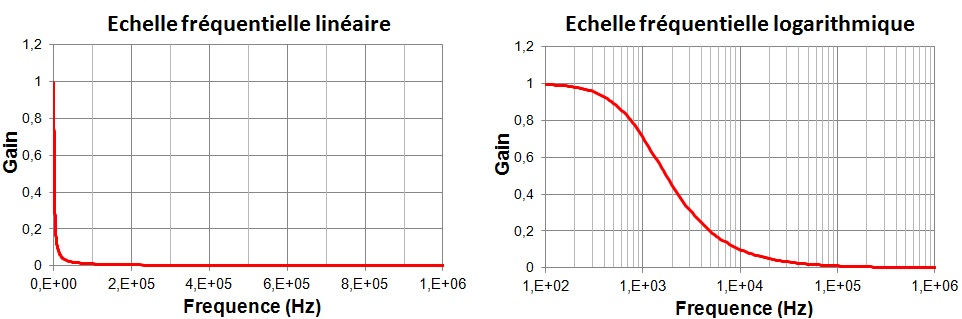
\includegraphics[scale=0.6]{images/Effet_Flin_log.jpg}
		\caption{Tracé du gain de la fonction de transfert d'un filtre passe-bas : échelle fréquentielle linéaire (à gauche) et logarithmique (à droite)}	
		\label{Fig:Effet_Flin_log} 
	\end{figure}
	\underline{Conseil pratique : comment tracer une échelle logarithmique ?}
	On définit tout d'abord le pas représentant une décade (par exemple 2 cm par décade). On considère que l'origine sera la valeur 1 (log10(1) = 0). La position de toute valeur par rapport à cette origine sera donnée par pas $\times log_{10}(valeur)$. Ainsi, la valeur 10 (une décade de plus que 1) sera située à 2 cm à droite de l'origine, 100 (deux décades de plus) sera située à 4 cm à droite de l'origine, tandis que 0.1 (une décade de moins) sera située à 2 cm à gauche de l'origine. La valeur 50 sera située à $2\times log10(50)$ = 3.4 cm à droite de l'origine.
	
	Une autre convention consiste à exprimer les gains en décibels, qui n'est rien d'autre qu'une représentation des valeurs sur une échelle logarithmique.. De part leur sélectivité en fréquence, les gains des filtres vont présenter des valeurs très variables en fonction de la fréquence. Pour les mêmes raisons que la représentation des fréquences, une échelle logarithmique pour le gain permettra d'apprécier avec la même résolution les faibles et les fortes valeurs de gain. La figure \ref{Fig:Effet_Ylin_dB} l'illustre, en reprenant l'exemple du tracé du gain du filtre précédent. Le tracé du gain sur une échelle linéaire ne permet pas de le mesurer précisément lorsqu'il atteint de faibles valeurs. A contrario, lorsqu'il est exprimé en dB, la mesure des faibles valeurs devient plus précise et il est possible de mettre en évidence des tendances particulières du gain. Par exemple, le gain de ce filtre décroit avec une pente de -20 dB par décade au-dessus de la fréquence de coupure, ce qui est typique d'un filtre passe-bas d'ordre 1. 
	\begin{equation}\label{}
	G_{dB} = 20 \cdot log(|H(f)|)
	\end{equation}
	
	\begin{figure}[h!]
		\centering
		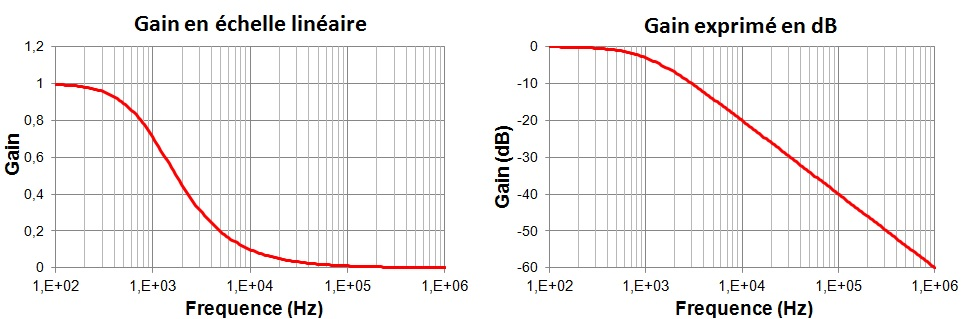
\includegraphics[scale=0.6]{images/Effet_Ylin_dB.jpg}
		\caption{Tracé du gain de la fonction de transfert d'un filtre passe-bas : échelle linéaire (à gauche) et en décibel (à droite)}	
		\label{Fig:Effet_Ylin_dB} 
	\end{figure}
	
	\begin{minipage}[l]{0.4\linewidth}
		Il n'y a pas de convention particulière pour le déphasage, qui peut être exprimé en radians ou en degrés. La figure ci-contre présente le diagramme de Bode du filtre précédent, montrant les tracés de l'évolution fréquentielle de son gain et de son déphasage. Le diagramme de Bode indique un déphasage dont la valeur diminue entre 0 et $-\frac{\pi}{2}$. Le déphasage étant négatif, le filtre introduit un retard.	
	\end{minipage} \hfill
	\begin{minipage}[c]{0.50\linewidth}
			%\centering
			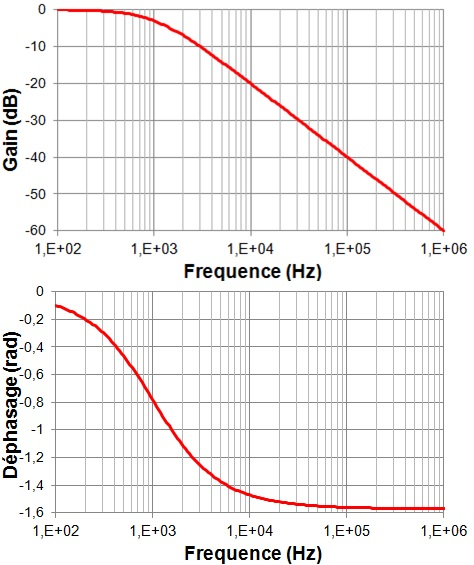
\includegraphics[scale=0.6]{images/Bode_passe-bas.jpg}
			%\caption{Diagramme de Bode d'un filtre passe-bas}	
			%\label{Fig:Bode_passe-bas} 	
	\end{minipage}
	
	
	
	\subsection{Exemples}
	J'en ai déjà fait un au-dessus.
	
	Filtres d'ordres 1 et 2 : Diagramme de Bode usuels et diagramme asymptotique
	Ordre 1 : passe-bas et passe-haut
	Ordre 2 : passe-bas, haut, passe-bande, coupe-bande (faire en TD ?)
	
	Filtre passe-bas d'ordre 1 :
	\begin{equation}\label{key}
	H(j\omega) = \frac{1}{1+j\frac{\omega}{\omega_{c}}}
	\end{equation}
	
	Filtre passe-haut d'ordre 1 :
	\begin{equation}\label{key}
	H(j\omega) = \frac{j\frac{\omega}{\omega_{c}}}{1+j\frac{\omega}{\omega_{c}}}
	\end{equation}
	
	Filtre passe-bas d'ordre 2 :
	\begin{equation}\label{key}
	H(j\omega) = \frac{1}{1+2\zeta j\frac{\omega}{\omega_{c}}+(j\frac{\omega}{\omega_{c}})^{2}}
	\end{equation}
	avec $\zeta$ le coefficient d'amortissement.
	\newline
	
	Filtre passe-haut d'ordre 2 :
	\begin{equation}\label{key}
	H(j\omega) = \frac{2\zeta j\frac{\omega}{\omega_{c}}}{1+2\zeta j\frac{\omega}{\omega_{c}}+(j\frac{\omega}{\omega_{c}})^{2}}
	\end{equation}
	
	Filtre passe-bande d'ordre 2 :
	\begin{equation}\label{key}
	H(j\omega) = \frac{(j\frac{\omega}{\omega_{c}})^{2}}{1+2\zeta j\frac{\omega}{\omega_{c}}+(j\frac{\omega}{\omega_{c}})^{2}}
	\end{equation}
	soit $Q = \frac{1}{2\zeta}$ le facteur de qualité. La bande passante de ce filtre est donnée par $\Delta f=\frac{f_{c}}{Q}$ où $f_{c}$ est la fréquence centrale du filtre.
	
	Filtre coupe-bande d'ordre 2 :
	\begin{equation}\label{key}
	H(j\omega) = \frac{1+(j\frac{\omega}{\omega_{c}})^{2}}{1+2\zeta j\frac{\omega}{\omega_{c}}+(j\frac{\omega}{\omega_{c}})^{2}}
	\end{equation}
	
	
	Mise en cascade filtre = Chainage de fonction de transfert
	
	\subsection{Gabarit}
	peut-être pas utile car on ne fera pas de synthèse de filtre.
	
	
	\underline{remarque : normalisation des fréquences :}
	Un filtre de nature donnée présentera toujours la même forme de gabarit. Seule la ou les fréquences de coupure changeront selon les propriétés du filtre. Pour disposer d'une représentation indépendante de la fréquence de coupure, il est courant de représenter l'axe des fréquences sous la forme d'une fréquence normalisée. Cette normalisation se fait par rapport à une fréquence de référence, généralement la fréquence coupure du filtre. Ainsi, le même gabarit peut être utilisé pour plusieurs filtres présentant différentes fréquences de coupure. Si l'axe fréquentiel est exprimé en pulsation, la normalisation se fera de la même manière.
	\begin{equation}\label{key}
	f_{norm} = \frac{f}{f_{c}}
	\end{equation}
	\begin{equation}\label{key}
	\omega_{norm} = \frac{\omega}{\omega_{c}}
	\end{equation}
	
	\begin{figure}[h!]
		\centering
		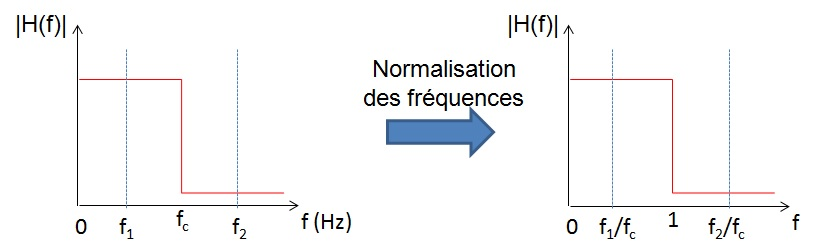
\includegraphics[scale=0.6]{images/freq_norm.jpg}
		\caption{Normalisation des fréquences}	
		\label{Fig:freq_norm} 
	\end{figure}

	\section{Les principales caractéristiques d'un filtr}e
	Lorsqu'on analyse un filtre ou lorsqu'on cherche à le dimensionner, plusieurs caractéristiques sont étudiées. Celles-ci définissent le comportement fréquentiel global. Nous allons les définir ici. 
	\begin{itemize}
		\item gain : le gain est dépendant de la fréquence. Néanmoins, on peut spécifier une valeur unique, qui correspond généralement à la valeur maximale du gain.
		\item fréquence(s) de coupure : celles-ci correspondent à des fréquences auxquelles le gain présente un changement de tendance. Dans la pratique, on considère un critère d'atténuation du gain de -3 dB (soit une division du gain par $\sqrt{2}$). On appelle fréquence de coupure (en toute rigueur fréquence de coupure à -3dB) d’un filtre toute fréquence positive ou nulle $f_{c}$ vérifiant :
	\end{itemize}
	\begin{equation}\label{key}
	|H(f_{c})|=\frac{\underset{\forall f \in \mathbb{R}^{+}}{max}(|H(f)|)}{\sqrt{2}} \Rightarrow~G_{dB}(f_{c})=\underset{\forall f \in \mathbb{R}^{+}}{max}(G_{dB}(f))-3
	\end{equation}
	Tout filtre admet alors une ou plusieurs fréquences de coupures : un filtre de gabarit passe-bas ou de gabarit passe-haut n’a qu’une fréquence de coupure, tandis qu’un filtre passe-bande ou coupe-bande classique a deux fréquences de coupure.
	\begin{itemize}
		\item bande passante : la sélectivité du filtre est donnée par sa bande passante. Il s'agit de la plage de fréquence sur laquelle l'atténuation est faible. Elle est délimitée par deux fréquences, définies selon un critère d'atténuation par rapport au gain maximal obtenu dans la bande passante. Un critère courant consiste à considérer une atténuation de -3 dB. La bande passante est donc la bande de fréquence où le gain reste compris entre sa valeur maximale et sa valeur maximale atténuée de 3 dB. On définit la bande passante d’un filtre comme l’ensemble des fréquences f de $\mathbb{R}^{+}$ pour lesquelles le module de la fonction de transfert demeure au moins égal à $\frac{1}{\sqrt{2}}$ fois sa valeur maximale. 
		La bande passante spécifie donc le domaine de fréquences à l’intérieur duquel le gain du filtre demeure plus ou moins constant, ou du moins ne chute pas de plus de 3 dB. Elle donne ainsi la plage de fréquences que le filtre va laisser passer, d’où son nom de bande passante ! La bande passante d’un filtre est constituée d’un ou plusieurs intervalles de $\mathbb{R}^{+}$, les bornes de ces intervalles étant données par les fréquences de coupure du filtre. Par exemple, la bande passante d’un filtre passe-bas est de la forme [0; fc] où fc est l’unique fréquence de coupure, tandis que la bande passante d’un filtre passe-haut est de la forme [fc;+1] ; la bande passante d’un filtre passe-bande classique (i.e. avec une seule bande passante) est de la forme [fc1; fc2] où fc1 et fc2 sont les deux fréquences de coupure, tandis que la bande passante d’un filtre coupe-bande classique (i.e. avec une seule bande coupée) est de la forme [0; fc1] [ [fc2;+1].
		\item équivalent bande passante pour un coupe bande
		\item pente de variation : lié à l'ordre
		\item fréquence(s) de résonance et d'antirésonance
		
	\end{itemize}
	
	
	\section{Les différents types de filtres}
	On classifie les filtres en quatre types selon la forme de leur gabarit : un filtre passe-bas laisse passer les basses fréquences (i.e. celles proches de la fréquence nulle) et atténue les hautes fréquences (i.e. celles grandes en valeur absolue), à l’inverse d’un filtre passe-haut ; le rôle d’un filtre passe-bande est de laisser passer uniquement les fréquences contenues dans un intervalle donné de fréquences, en atténuant toutes les autres, tandis qu’à l’inverse le rôle d’un filtre coupe-bande est de supprimer toutes les fréquences contenues dans un intervalle donné en laissant passer toutes les autres. Les gabarits des différents types de filtres idéaux :
	
	
	Les filtres physiquement réalisables sont néanmoins caractérisés par :
	\begin{itemize}
		\item des pentes de variation de gain finis, liées à l'ordre du filtre
	\end{itemize}
	
	
	\section{Méthodes simples d'analyse de fonction de transfert}
	Dans la pratique, on s'intéresse souvent à la tendance du comportement, ou au comportement autour de point spécifique.
	
	Comportement asymptotique : les valeurs des pentes en fonction des ordres. Ordre 1 : *10 : +20 dB. Ordre 2 : * 10 : + 40 dB. Ordre N : *10 : 20*N dB. On parlera de pente en dB/dec.
	
	Analyse aux résonances et anti-résonances
	
	
	\section{Ce qu'il faut retenir}
	Une question qui se pose maintenant : nous avons vu que l'étude des systèmes LTI, dont les filtres, est particulièrement simplifiée dans le domaine fréquentiel, via l'analyse harmonique. La transformée de Laplace constitue un outil permettant d'extraire la fonction de transfert des systèmes LTI.
	Notre objectif est de déterminer comment un filtre agit sur un signal d'entrée quelconque. Les signaux sont généralement acquis dans le domaine temporel. Pour analyser l'effet du filtre, il est donc nécessaire de calculer la représentation fréquentielle du signal au préalable. Pour cela, nous allons utiliser la transformée de Fourier qui sera présentée dans les deux prochains chapitres. Comme nous le verrons, cet outil est très proche de la transformée de Laplace, qui constitue une généralisation. 
	
	
	\section{Exercices }
	Un exercice sur un filtre déphaseur pur (passe-tout). 
	
	
	Exo bêbête : on présente le contenu fréquentiel d'un signal bruité, en indiquant la bande passante du signal utile. Quel type de filtre faut-il mettre ? Quel ordre ?
	
	Filtre anti-glitch
	Soit une perturbation, que l'on considère d'abord comme une impulsion rectangulaire de largeur tau, puis d'impulsion double exponentielle.
	
	Dans chaque cas, calculez la transformée de Laplace des signaux.
	
	Exprimez l'amplitude maximale atteinte par ces signaux.
	
	On applique un filtre passe-bas d'ordre 1 d'expression … Calculez la réponse du filtre dans le domaine de Laplace pour les deux types d'excitation.
	
	Calculez les amplitudes maximales des signaux. Quelle est l'influence du paramètre Fc.
	
	Ce filtre est placée sur une ligne de signal électrique de fréquence … Proposez une valeur pour Fc.
	
	\newpage
	
\chapter{Séries de Fourier}


	\newpage
	
\chapter{Transformée de Fourier}

	\newpage
	
\chapter{Analyse des systèmes et des signaux dans le domaine temporel}
	
	Jusque-là, nous avons principalement calculé la réponse de systèmes LTI en passant par le domaine fréquentiel, en utilisant les notions de fonctions de transfert, de transformée de Fourier et de Laplace. Cette approche permettait de calculer facilement cette réponse.
	Tous les calculs auraient pu être effectué en restant dans le domaine temporel à partir de la réponse impulsionnelle du système, que nous avions introduite au chapitre B. Nous l'avions laissé de côté momentanément car son utilisation passait par un calcul relativement complexe appelé produit de convolution. Nous allons le détailler dans ce chapitre.
	Nous pourrions croire que nous sommes en train de présenter un nouvel outil pour analyser l'effet d'un même système LTI. Nous allons voir au contraire que les concepts de fonction de transfert et de réponse impulsionnelle sont intimement liées.
	L'analyse temporelle présente de nombreux intérêts que nous allons aussi aborder. Par exemple, la notion de corrélation, permettant de mesurer le degré de ressemblance entre deux signaux. Cette dernière notion ne permettra d'aborder un des aspects que nous n'avons pas encore abordé : la manière dont l'énergie est répartie dans le domaine fréquentiel et l'impact du système sur le transfert d'énergie ou de puissance. A partir des relations dans le domaine temporel et fréquentiel, nous pourrons aborder ces questions.
	
	\section{Réponse impulsionnelle}
	Comme nous l'avons vu dans le chapitre 2, il s'agit de la réponse d'un système LTI à une excitation impulsionnelle élémentaire, modélisée par une impulsion de Dirac. Sa connaissance permet de déterminer la réponse du système quelle que soit l'excitation appliquée à l'aide de la relation suivante, présentée au chapitre 2.
	\begin{equation}\label{Calcul_reponse_temporel_causal}
	y(t) = \int_{0}^{+ \infty} x(\tau) \cdot h(t-\tau)d\tau = x*h(t)
	\end{equation}
	\vspace{1\baselineskip}
	La réponse impulsionnelle et la fonction de transfert d'un système sont reliées par la transformée de Laplace. Plusieurs moyens permettent de le démontrer. Le plus simple consiste à exploiter le lien entre la multiplication et le produit de convolution : un produit de convolution dans le domaine temporel est équivalent à une multiplication dans le domaine fréquentiel.
	\begin{equation}\label{}
	y(t) =  h*x(t) ~\longleftrightarrow~Y(p)=H(p)\cdot X(p)
	\end{equation}
	
	Dans la prochaine partie, nous allons détailler les propriétés du produit de convolution et voir comment le mettre en œuvre pour résoudre l'équation \ref{Calcul_reponse_temporel_causal}.
	
	\section{Produit de convolution}
	\subsection{Définition}
	Soient deux fonctions x(t) et y(t) définis sur ... Le produit de convolution est donné par l'équation \ref{Convolution}.
	\begin{equation}\label{Convolution}
	x*y(t) = \int_{-\infty}^{+ \infty} x(\tau) \cdot y(t-\tau)d\tau 
	\end{equation}
	
	\subsection{Propriétés}
	Le tableau ci-dessous résume les principales propriétés du produit de convolution.
		
	\subsection{Mise en œuvre du produit de convolution}
	Voyons la démarche pour calculer manuellement un produit de convolution. Nous considérons un système causal dont on connait la réponse impulsionnelle h(t) ainsi que l'excitation x(t).
	
	
	
	
\chapter*{Annexe - complexe}
	Vecteur de Fresnel.
	
	\underline{Phaseur :}
	Considérons le cas d'une excitation sinusoïdale pure. La grandeur
	complexe $ \hat{X} =|X| \cdot exp(j \theta(t)) $ représente un vecteur, appelé vecteur de Fresnel, amplitude complexe ou phaseur. Il
	s'agit d'un vecteur tournant dans le plan complexe à la fréquence $\omega$. La
	projection de ce phaseur sur l'axe réel donne la valeur instantanée
	prise par le signal.
	
	
\end{document}
